% Options for packages loaded elsewhere
\PassOptionsToPackage{unicode}{hyperref}
\PassOptionsToPackage{hyphens}{url}
%
\documentclass[
]{book}
\usepackage{lmodern}
\usepackage{amssymb,amsmath}
\usepackage{ifxetex,ifluatex}
\ifnum 0\ifxetex 1\fi\ifluatex 1\fi=0 % if pdftex
  \usepackage[T1]{fontenc}
  \usepackage[utf8]{inputenc}
  \usepackage{textcomp} % provide euro and other symbols
\else % if luatex or xetex
  \usepackage{unicode-math}
  \defaultfontfeatures{Scale=MatchLowercase}
  \defaultfontfeatures[\rmfamily]{Ligatures=TeX,Scale=1}
\fi
% Use upquote if available, for straight quotes in verbatim environments
\IfFileExists{upquote.sty}{\usepackage{upquote}}{}
\IfFileExists{microtype.sty}{% use microtype if available
  \usepackage[]{microtype}
  \UseMicrotypeSet[protrusion]{basicmath} % disable protrusion for tt fonts
}{}
\makeatletter
\@ifundefined{KOMAClassName}{% if non-KOMA class
  \IfFileExists{parskip.sty}{%
    \usepackage{parskip}
  }{% else
    \setlength{\parindent}{0pt}
    \setlength{\parskip}{6pt plus 2pt minus 1pt}}
}{% if KOMA class
  \KOMAoptions{parskip=half}}
\makeatother
\usepackage{xcolor}
\IfFileExists{xurl.sty}{\usepackage{xurl}}{} % add URL line breaks if available
\IfFileExists{bookmark.sty}{\usepackage{bookmark}}{\usepackage{hyperref}}
\hypersetup{
  pdftitle={Conducting Monte Carlo Simulations in R},
  pdfauthor={Okan Bulut},
  hidelinks,
  pdfcreator={LaTeX via pandoc}}
\urlstyle{same} % disable monospaced font for URLs
\usepackage{color}
\usepackage{fancyvrb}
\newcommand{\VerbBar}{|}
\newcommand{\VERB}{\Verb[commandchars=\\\{\}]}
\DefineVerbatimEnvironment{Highlighting}{Verbatim}{commandchars=\\\{\}}
% Add ',fontsize=\small' for more characters per line
\usepackage{framed}
\definecolor{shadecolor}{RGB}{248,248,248}
\newenvironment{Shaded}{\begin{snugshade}}{\end{snugshade}}
\newcommand{\AlertTok}[1]{\textcolor[rgb]{0.94,0.16,0.16}{#1}}
\newcommand{\AnnotationTok}[1]{\textcolor[rgb]{0.56,0.35,0.01}{\textbf{\textit{#1}}}}
\newcommand{\AttributeTok}[1]{\textcolor[rgb]{0.77,0.63,0.00}{#1}}
\newcommand{\BaseNTok}[1]{\textcolor[rgb]{0.00,0.00,0.81}{#1}}
\newcommand{\BuiltInTok}[1]{#1}
\newcommand{\CharTok}[1]{\textcolor[rgb]{0.31,0.60,0.02}{#1}}
\newcommand{\CommentTok}[1]{\textcolor[rgb]{0.56,0.35,0.01}{\textit{#1}}}
\newcommand{\CommentVarTok}[1]{\textcolor[rgb]{0.56,0.35,0.01}{\textbf{\textit{#1}}}}
\newcommand{\ConstantTok}[1]{\textcolor[rgb]{0.00,0.00,0.00}{#1}}
\newcommand{\ControlFlowTok}[1]{\textcolor[rgb]{0.13,0.29,0.53}{\textbf{#1}}}
\newcommand{\DataTypeTok}[1]{\textcolor[rgb]{0.13,0.29,0.53}{#1}}
\newcommand{\DecValTok}[1]{\textcolor[rgb]{0.00,0.00,0.81}{#1}}
\newcommand{\DocumentationTok}[1]{\textcolor[rgb]{0.56,0.35,0.01}{\textbf{\textit{#1}}}}
\newcommand{\ErrorTok}[1]{\textcolor[rgb]{0.64,0.00,0.00}{\textbf{#1}}}
\newcommand{\ExtensionTok}[1]{#1}
\newcommand{\FloatTok}[1]{\textcolor[rgb]{0.00,0.00,0.81}{#1}}
\newcommand{\FunctionTok}[1]{\textcolor[rgb]{0.00,0.00,0.00}{#1}}
\newcommand{\ImportTok}[1]{#1}
\newcommand{\InformationTok}[1]{\textcolor[rgb]{0.56,0.35,0.01}{\textbf{\textit{#1}}}}
\newcommand{\KeywordTok}[1]{\textcolor[rgb]{0.13,0.29,0.53}{\textbf{#1}}}
\newcommand{\NormalTok}[1]{#1}
\newcommand{\OperatorTok}[1]{\textcolor[rgb]{0.81,0.36,0.00}{\textbf{#1}}}
\newcommand{\OtherTok}[1]{\textcolor[rgb]{0.56,0.35,0.01}{#1}}
\newcommand{\PreprocessorTok}[1]{\textcolor[rgb]{0.56,0.35,0.01}{\textit{#1}}}
\newcommand{\RegionMarkerTok}[1]{#1}
\newcommand{\SpecialCharTok}[1]{\textcolor[rgb]{0.00,0.00,0.00}{#1}}
\newcommand{\SpecialStringTok}[1]{\textcolor[rgb]{0.31,0.60,0.02}{#1}}
\newcommand{\StringTok}[1]{\textcolor[rgb]{0.31,0.60,0.02}{#1}}
\newcommand{\VariableTok}[1]{\textcolor[rgb]{0.00,0.00,0.00}{#1}}
\newcommand{\VerbatimStringTok}[1]{\textcolor[rgb]{0.31,0.60,0.02}{#1}}
\newcommand{\WarningTok}[1]{\textcolor[rgb]{0.56,0.35,0.01}{\textbf{\textit{#1}}}}
\usepackage{longtable,booktabs}
% Correct order of tables after \paragraph or \subparagraph
\usepackage{etoolbox}
\makeatletter
\patchcmd\longtable{\par}{\if@noskipsec\mbox{}\fi\par}{}{}
\makeatother
% Allow footnotes in longtable head/foot
\IfFileExists{footnotehyper.sty}{\usepackage{footnotehyper}}{\usepackage{footnote}}
\makesavenoteenv{longtable}
\usepackage{graphicx,grffile}
\makeatletter
\def\maxwidth{\ifdim\Gin@nat@width>\linewidth\linewidth\else\Gin@nat@width\fi}
\def\maxheight{\ifdim\Gin@nat@height>\textheight\textheight\else\Gin@nat@height\fi}
\makeatother
% Scale images if necessary, so that they will not overflow the page
% margins by default, and it is still possible to overwrite the defaults
% using explicit options in \includegraphics[width, height, ...]{}
\setkeys{Gin}{width=\maxwidth,height=\maxheight,keepaspectratio}
% Set default figure placement to htbp
\makeatletter
\def\fps@figure{htbp}
\makeatother
\setlength{\emergencystretch}{3em} % prevent overfull lines
\providecommand{\tightlist}{%
  \setlength{\itemsep}{0pt}\setlength{\parskip}{0pt}}
\setcounter{secnumdepth}{5}
\usepackage{booktabs}
\usepackage{amsthm}
\makeatletter
\def\thm@space@setup{%
  \thm@preskip=8pt plus 2pt minus 4pt
  \thm@postskip=\thm@preskip
}
\makeatother

\usepackage{booktabs}
\usepackage{longtable}
\usepackage{array}
\usepackage{multirow}
\usepackage{wrapfig}
\usepackage{float}
\usepackage{colortbl}
\usepackage{pdflscape}
\usepackage{tabu}
\usepackage{threeparttable}
\usepackage{threeparttablex}
\usepackage[normalem]{ulem}
\usepackage{makecell}
\usepackage[]{natbib}
\bibliographystyle{apalike}

\title{Conducting Monte Carlo Simulations in R}
\author{Okan Bulut}
\date{University of Alberta, \href{mailto:bulut@ualberta.ca}{\nolinkurl{bulut@ualberta.ca}}}

\begin{document}
\maketitle

{
\setcounter{tocdepth}{1}
\tableofcontents
}
\hypertarget{intro}{%
\chapter{Introduction}\label{intro}}

\includegraphics{figure/david-rangel-4m7gmLNr3M0-unsplash.jpg}

\hypertarget{overview}{%
\section{Overview}\label{overview}}

Both researchers and practitioners often use Monte Carlo simulations to answer a variety of research questions. Over the past decade, \texttt{R} \citep{R-base} has been one of the most popular programming languages for conducting Monte Carlo simulation studies. \texttt{R} (\url{https://www.r-project.org/}) is a free, open-source programming language for statistical computing and data visualization. Both built-in functions and many user-created packages in \texttt{R} allow researchers and practitioners to design and implement a very simple to very comprehensive simulation studies.

This short book will explain the \textbf{major} steps in conducting Monte Carlo simulations using \texttt{R}. Here is the outline of the book\footnote{This book was created using the \texttt{bookdown} \citep{R-bookdown} and \texttt{knitr} \citep{R-knitr} packages.}:

\begin{longtable}[]{@{}ll@{}}
\toprule
Part & Description\tabularnewline
\midrule
\endhead
\textbf{1} & \textbf{Introduction} ~~\tabularnewline
& Why Simulations?\tabularnewline
& Typical Simulation Scenarios\tabularnewline
& Additional Resources\tabularnewline
\textbf{2} & \textbf{Designing Simulations} ~~\tabularnewline
& Simulation Factors\tabularnewline
& Evaluation Criteria\tabularnewline
& Other Design Elements\tabularnewline
\textbf{3} & \textbf{Running Simulation} ~~\tabularnewline
& Custom Functions\tabularnewline
& Debugging the Code\tabularnewline
& Putting the Functions Together\tabularnewline
& Benchmarking\tabularnewline
\textbf{4} & \textbf{Summarizing Simulation Results} ~~\tabularnewline
& Tables and Figures\tabularnewline
& Exporting the Results\tabularnewline
\bottomrule
\end{longtable}

\hypertarget{why-simulations}{%
\section{Why Simulations?}\label{why-simulations}}

There are many reasons to conduct Monte Carlo simulations. Researchers and practitioners often choose to simulate data instead of collecting empirical data because:

\begin{itemize}
\tightlist
\item
  it is \textbf{impractical} and \textbf{costly} to collect empirical data while manipulating several conditions
\item
  it is not possible to investigate the \textbf{real impact} of the study conditions without knowing the characteristics of the target population as well as the variables of interest.
\item
  it is more difficult to deal with empirical data because it typically includes \textbf{missingness} -- which may be in large amounts and nonrandom.
\end{itemize}

\hypertarget{typical-simulation-scenarios}{%
\section{Typical Simulation Scenarios}\label{typical-simulation-scenarios}}

We can use Monte Carlo simulations to answer various research questions. Typical research questions in which Monte Carlo simulations can be useful are:

\begin{itemize}
\tightlist
\item
  Does a particular type of estimation (e.g., maximum likelihood) yield accurate results?

  \begin{itemize}
  \tightlist
  \item
    What is the level of bias?
  \item
    What is the standard error of estimates?
  \item
    What conditions would affect the accuracy of the estimation?
  \item
    Does the estimation remain robust when assumptions are violated?
  \end{itemize}
\item
  Which estimation method (e.g., maximum likelihood, EAP, and MAP) is more accurate?

  \begin{itemize}
  \tightlist
  \item
    Do the performances of these methods vary by different conditions?
  \item
    Which estimator, method, or model is the most robust?
  \end{itemize}
\item
  Can a statistical method or model (e.g., logistic regression) successfully detect a value of interest (e.g., differential item functioning)?

  \begin{itemize}
  \tightlist
  \item
    How accurate is the method when the null hypothesis is \emph{false}?
  \item
    How accurate is the method when the null hypothesis is \emph{true}?
  \end{itemize}
\end{itemize}

\hypertarget{additional-resources}{%
\section{Additional Resources}\label{additional-resources}}

If you are interested in learning more about Monte Carlo simulations, there are many online resources available. Some of these resources include:

\begin{itemize}
\tightlist
\item
  \citet{bulut2017}'s article: \href{https://dergipark.org.tr/en/download/article-file/343265}{Monte Carlo Simulation Studies in Item Response Theory with the R Programming Language}
\item
  \citet{hallgren_2013}'s article: \href{http://tqmp.org/Content/vol09-2/p043/p043.pdf}{Conducting Simulation Studies in the R Programming Environment}
\item
  Roger Peng's online book: \href{https://bookdown.org/rdpeng/rprogdatascience/}{R Programming for Data Science}. In the book, \href{https://bookdown.org/rdpeng/rprogdatascience/simulation.html}{Chapter 20} specifically focuses on simulations in R.
\item
  The \texttt{SimDesign} \citep{R-SimDesign} package in \texttt{R}. For examples of \texttt{SimDesign}, you can check out its Wiki page: \url{https://github.com/philchalmers/SimDesign/wiki}
\item
  There is also another \texttt{R} package called \texttt{MonteCarlo} \citep{R-MonteCarlo} for more general simulation studies.
\end{itemize}

\hypertarget{design}{%
\chapter{Designing Simulations}\label{design}}


\includegraphics{figure/galymzhan-abdugalimov-ICW6QYOcdlg-unsplash.jpg}

To better explain the steps of conducting a Monte Carlo simulation study, let's assume a hypothetical research scenario in which a researcher wants to examine item parameter estimation in item response theory (IRT). Here the researcher aims to determine the robustness of parameter estimation for the 3PL model, especially when the sample size is small.

\hypertarget{simulation-factors}{%
\section{Simulation Factors}\label{simulation-factors}}

The researcher can investigate the impact of several factors (i.e., conditions) within the same study but the goal is to create a feasible study with the factors that are essential for this study. Therefore, the following factors are selected:

\begin{itemize}
\tightlist
\item
  Test length (10, 15, 20, or 25 items)
\item
  Sample size (250, 500, 750, or 1000 examinees)
\item
  Whether or not the guessing (c) parameter should be fixed for all items (e.g., \(c = 0.16\))
\end{itemize}

Let's see the total number of conditions from these factors:

4 (test length) x 4 (sample size) x 2 (fixed guessing or free estimation) = 32 conditions

This calculation assumes that these factors are \textbf{fully crossed}. Two factors are fully crossed when each level of one factor occurs in combination with each level of the other factor. However, some factors may not be crossed with the other factors. These are called \textbf{nested} factors. Two factors are nested when each level of a factor occurs in combination with different levels of another factor (see \href{https://besjournals.onlinelibrary.wiley.com/doi/full/10.1111/j.2041-210x.2012.00251.x}{Schielzeth and Nakagawa's paper} for more information about crossed and nested factors).

\hypertarget{evaluation-criteria}{%
\section{Evaluation Criteria}\label{evaluation-criteria}}

The researcher is interested in \textbf{accuracy}. Therefore, we have to use several measures of accuracy to evaluate the simulation results. Some of these measures (i.e., indices) include:

\begin{itemize}
\item
  \textbf{Bias:} \(bias = \frac{1}{R} \Sigma_{r=1}^{R} (\hat{x_r}-x)\), where \(R\) is the number of replications, \(\hat{x_r}\) is the estimated value of the parameter, and \(x\) is the true value of the parameter. Bias, which can be either positive or negative, should be close to zero for higher accuracy.
\item
  \textbf{Root-mean square error (RMSE):} \(RMSE = \sqrt{\frac{1}{R} \Sigma_{r=1}^{R} (\hat{x_r}-x)^2}\), where \(R\) is the number of replications, \(\hat{x_r}\) is the estimated value of the parameter, and \(x\) is the true value of the parameter. RMSE, which is either zero or a positive value, should be close to zero for higher accuracy.
\item
  \textbf{(Pearson) Correlation:} \(\rho(x,\hat{x}) = \frac{\text{cov}(x,\hat{x})}{\sigma_x \sigma_{\hat{x}}}\), where \(\hat{x_r}\) is the estimated value of the parameter, \(x\) is the true value of the parameter, the numerator is the covariance of the two parameters, and the denominator is the product of their standard deviations. Correlation should be closer to 1 as the accuracy increases.
\end{itemize}

Note that there are other types of evaluation criteria, such as power, type I error, relative efficiency, precision, and recall. In this study, the accuracy measures listed above should be adequate for evaluating the accuracy of estimated item paramaters. We will discuss how the simulation results with these evaluation criteria can be summarized and presented in Part \ref{summarise} of this book.

\hypertarget{other-design-elements}{%
\section{Other Design Elements}\label{other-design-elements}}

\textbf{Item and ability parameters:} The researcher must use either a fixed set of item parameters from an existing instrument or simulated item parameters similar to those from an existing instrument. Thus, the researcher uses the distributions provided in \citet{casa2015}'s article based on a 2008 National Mathematics Assessment:

\begin{itemize}
\tightlist
\item
  \(a \sim N(1.13, 0.25)\)
\item
  \(b \sim N(0.21, 0.51)\)
\item
  \(c \sim N(0.16, 0.05)\)
\end{itemize}

For the ability distribution, ability values are drawn from a normal distribution, \(\theta \sim N(0, 1)\).

\textbf{Number of replications:} The number of replications should be adequate to create enough variation in the simulation. The higher the number of replications, the longer the simulation study will take. Therefore, it is important to choose a suitable number. Typically, 100 replications are enough for this type of simulation study. We can test this by increasing the number of iterations to 150 and check whether the overall results would change substantially.

\textbf{Replication mechanism:} In a typical Monte Carlo simulation study, the levels of simulation factors remain fixed, while the data, parameters, and other parts vary. In other words, these are the parts that we actually simulate. For the sake of simplicity, some of these parts can be generated once while the other parts continuously change from one replication to another. In this study, the researcher does not have a specific set of item parameters to test. Instead, the goal of the study is more general: investigating the impact of the identified simulation factors on item parameter estimation. Therefore, unique sets of item parameters, ability values, and response data can be generated with each replication.

\hypertarget{run}{%
\chapter{Running Simulations}\label{run}}


\includegraphics{figure/john-schnobrich-yFbyvpEGHFQ-unsplash.jpg}

The secret of building a successful Monte Carlo simulation is to write several custom functions that work efficiently and more importantly -- \textbf{correctly}. Then, we can:

\begin{itemize}
\tightlist
\item
  combine the custom functions within a single function and run the simulations using this function with nested loops, or
\item
  write several nested loops that run each custom function independently and carry its output to the next function.
\end{itemize}

As we put the simulation functions together, we should be aware of potential errors that could either produce incorrect results or interrupt the execution of the simulation at different stages. Therefore, it is important to check all the functions carefully and patiently before running the simulations. Adding either notifications or diagnostic messages into the functions is also quite helpful for debugging problems that might occur in the functions.

Once all the simulation functions are checked, the next step is determine how to run the simulations as efficiently as possible. Loops are particularly slow in \texttt{R} when it comes to handling heavy computations and data operations. The \texttt{apply()} function collection including \texttt{apply()}, \texttt{sapply()}, and \texttt{lapply()} can help users avoid the loops and perform many computations and data operations very efficiently in \texttt{R}. For users who want to run their simulations with loops, parallel computing in \texttt{R} is also an excellent way to make the simulations faster. Regardless of which of these methods has been selected, it is useful to check running time of \texttt{R} codes -- which is also known as \textbf{benchmarking}. We will discuss all of these steps in the remainder of Part \ref{run}.

\hypertarget{custom-functions}{%
\section{Custom Functions}\label{custom-functions}}

Writing custom functions does \textbf{not} mean that we must write every single algorithm from scratch. Instead, it means that we bring several functions (either new or existing) together so that they run the analysis that we want and return the results in the way we prefer. Going back to the hypothetical simulation scenario that we introducted in Part \ref{intro}, the researcher needs several custom functions for:

\begin{enumerate}
\def\labelenumi{\arabic{enumi}.}
\tightlist
\item
  Generating response data
\item
  Estimating item parameters
\item
  Calculating bias, RMSE, and correlation
\end{enumerate}

In the first function, we want the function to generate item parameters based on the parameter distributions that we have mentioned in Part \ref{design} and to use these parameters to generate dichotomous response data following the 3PL model. We call this function \texttt{generate\_data}. Our function has several arguments based on the simulation factors: \texttt{nitem} for the number of items, \texttt{nexaminee} for the number of examinees, and \texttt{seed} that allows us to control the random number generation. Setting the seed is very important in Monte Carlo simulations because it enables the reproducibility of simulation results. When we run the same function using the same seeds in the future, we should be able to generate the same parameters and response data.

To generate responses, we will use the \texttt{sim} function from the \texttt{irtoys} package \citep{R-irtoys}. We could make \texttt{irtoys} a required package for our custom function, using \texttt{require("irtoys")}. This would activate the package every time we use \texttt{generate\_data}. However, some packages can mask functions from other packages with the same names, when they are activated together within the same \texttt{R} session. Therefore, it is better to call the exact function that we want to use, instead of activating the entire package. Here we use \texttt{irtoys::sim} to call the \texttt{sim} function from \texttt{irtoys}.

Note that the three arguments, \texttt{nitem}, \texttt{nexaminee}, and \texttt{seed}, in the \texttt{generate\_data} function are \textbf{required}. That is, all of these arguments must be specified as we run the simulations. This might create some problems in the simulation. We will talk about this in the debugging section later on.

\begin{Shaded}
\begin{Highlighting}[]
\NormalTok{generate_data <-}\StringTok{ }\ControlFlowTok{function}\NormalTok{(nitem, nexaminee, seed) \{}
  \CommentTok{# Set the seed }
  \KeywordTok{set.seed}\NormalTok{(seed)}

  \CommentTok{# Generate item parameters}
\NormalTok{  itempar <-}\StringTok{ }\KeywordTok{cbind}\NormalTok{(}
    \KeywordTok{rnorm}\NormalTok{(nitem, }\DataTypeTok{mean =} \FloatTok{1.13}\NormalTok{, }\DataTypeTok{sd =} \FloatTok{0.25}\NormalTok{)}\OperatorTok{*}\FloatTok{1.702}\NormalTok{, }\CommentTok{#a}
    \KeywordTok{rnorm}\NormalTok{(nitem, }\DataTypeTok{mean =} \FloatTok{0.21}\NormalTok{, }\DataTypeTok{sd =} \FloatTok{0.51}\NormalTok{)}\OperatorTok{*}\FloatTok{1.702}\NormalTok{, }\CommentTok{#b}
    \KeywordTok{rnorm}\NormalTok{(nitem, }\DataTypeTok{mean =} \FloatTok{0.16}\NormalTok{, }\DataTypeTok{sd =} \FloatTok{0.05}\NormalTok{))       }\CommentTok{#c}
  
  \CommentTok{# Generate ability parameters}
\NormalTok{  ability <-}\StringTok{ }\KeywordTok{rnorm}\NormalTok{(nexaminee, }\DataTypeTok{mean =} \DecValTok{0}\NormalTok{, }\DataTypeTok{sd =} \DecValTok{1}\NormalTok{)}
  
  \CommentTok{# Generate response data according to the 3PL model}
\NormalTok{  respdata <-}\StringTok{ }\NormalTok{irtoys}\OperatorTok{::}\KeywordTok{sim}\NormalTok{(}\DataTypeTok{ip =}\NormalTok{ itempar, }\DataTypeTok{x =}\NormalTok{ ability)}
  \KeywordTok{colnames}\NormalTok{(respdata) <-}\StringTok{ }\KeywordTok{paste0}\NormalTok{(}\StringTok{"item"}\NormalTok{, }\DecValTok{1}\OperatorTok{:}\NormalTok{nitem)}
  
  \CommentTok{# Combine the generated values in a list}
\NormalTok{  data <-}\StringTok{ }\KeywordTok{list}\NormalTok{(}\DataTypeTok{itempar =}\NormalTok{ itempar,}
               \DataTypeTok{ability =}\NormalTok{ ability,}
               \DataTypeTok{seed =}\NormalTok{ seed,}
               \DataTypeTok{respdata =}\NormalTok{ respdata)}
  
  \CommentTok{# Return the simulated data}
  \KeywordTok{return}\NormalTok{(data)}
\NormalTok{\}}
\end{Highlighting}
\end{Shaded}

Our function saves the item parameters, ability parameters, simulated responses, and the seed for the \texttt{set.seed} argument. Let's see if our function returns what we asked for.

\begin{Shaded}
\begin{Highlighting}[]
\NormalTok{temp1a <-}\StringTok{ }\KeywordTok{generate_data}\NormalTok{(}\DataTypeTok{nitem =} \DecValTok{10}\NormalTok{, }\DataTypeTok{nexaminee =} \DecValTok{1000}\NormalTok{, }\DataTypeTok{seed =} \DecValTok{666}\NormalTok{)}
\KeywordTok{head}\NormalTok{(temp1a}\OperatorTok{$}\NormalTok{itempar)}
\KeywordTok{head}\NormalTok{(temp1a}\OperatorTok{$}\NormalTok{ability)}
\KeywordTok{head}\NormalTok{(temp1a}\OperatorTok{$}\NormalTok{respdata)}
\end{Highlighting}
\end{Shaded}

\begin{verbatim}
      [,1]    [,2]    [,3]
[1,] 2.244  2.2237 0.12540
[2,] 2.780 -1.1792 0.10085
[3,] 1.772  1.1080 0.22344
[4,] 2.786 -1.1357 0.14437
[5,] 0.980  0.4738 0.16153
[6,] 2.246  0.2916 0.08589
\end{verbatim}

\begin{verbatim}
[1]  0.7550 -0.6415  1.4311 -0.6246  0.2290  0.2632
\end{verbatim}

\begin{verbatim}
     item1 item2 item3 item4 item5 item6 item7 item8 item9 item10
[1,]     0     1     1     1     1     1     1     0     1      1
[2,]     0     1     1     1     1     0     0     0     0      0
[3,]     0     1     1     1     1     1     1     0     1      1
[4,]     0     1     0     0     0     0     0     0     1      0
[5,]     0     1     1     1     1     1     1     0     1      0
[6,]     0     1     1     1     0     1     0     1     0      1
\end{verbatim}

Our second function is the \texttt{mirt} function from the \texttt{mirt} package \citep{R-mirt}. We will create a custom function to be able to add a fixed guessing parameter and to extract the estimated item parameters. Here we will set \texttt{guess} as a negative value (e.g., -1), indicating that we want guessing to be freely estimated. However, if \texttt{guess} is greater than or equal to zero, then the guessing parameter will be fixed to this value in the function.

\begin{Shaded}
\begin{Highlighting}[]
\NormalTok{estimate_par <-}\StringTok{ }\ControlFlowTok{function}\NormalTok{(data, }\DataTypeTok{guess =} \DecValTok{-1}\NormalTok{) \{}
  \CommentTok{# If guessing is fixed}
  \ControlFlowTok{if}\NormalTok{(guess }\OperatorTok{>=}\StringTok{ }\DecValTok{0}\NormalTok{) \{}
    
    \CommentTok{# Model set up}
\NormalTok{    mod3PL <-}\StringTok{ }\NormalTok{mirt}\OperatorTok{::}\KeywordTok{mirt}\NormalTok{(data, }\CommentTok{# response data}
                         \DecValTok{1}\NormalTok{,    }\CommentTok{# unidimensional model}
                         \DataTypeTok{guess =}\NormalTok{ guess, }\CommentTok{# fixed guessing}
                         \DataTypeTok{verbose =} \OtherTok{FALSE}\NormalTok{, }\CommentTok{# Don't print verbose}
                         \CommentTok{# Increase the number of EM cycles}
                         \CommentTok{# Turn off estimation messages}
                         \DataTypeTok{technical =} \KeywordTok{list}\NormalTok{(}\DataTypeTok{NCYCLES =} \DecValTok{1000}\NormalTok{,}
                                          \DataTypeTok{message =} \OtherTok{FALSE}\NormalTok{)) }
\NormalTok{  \} }\ControlFlowTok{else}\NormalTok{ \{}
\NormalTok{    mod3PL <-}\StringTok{ }\NormalTok{mirt}\OperatorTok{::}\KeywordTok{mirt}\NormalTok{(data, }\CommentTok{# response data}
                         \DecValTok{1}\NormalTok{,    }\CommentTok{# unidimensional model}
                         \DataTypeTok{itemtype =} \StringTok{"3PL"}\NormalTok{, }\CommentTok{# IRT model}
                         \DataTypeTok{verbose =} \OtherTok{FALSE}\NormalTok{, }\CommentTok{# Don't print verbose}
                         \CommentTok{# Increase the number of EM cycles}
                         \CommentTok{# Turn off estimation messages}
                         \DataTypeTok{technical =} \KeywordTok{list}\NormalTok{(}\DataTypeTok{NCYCLES =} \DecValTok{1000}\NormalTok{,}
                                          \DataTypeTok{message =} \OtherTok{FALSE}\NormalTok{)) }
\NormalTok{  \}}
  
  \CommentTok{# Extract item parameters in typical IRT metric}
\NormalTok{  itempar_est <-}\StringTok{ }\KeywordTok{as.data.frame}\NormalTok{(mirt}\OperatorTok{::}\KeywordTok{coef}\NormalTok{(mod3PL, }\DataTypeTok{IRTpars =} \OtherTok{TRUE}\NormalTok{, }\DataTypeTok{simplify =} \OtherTok{TRUE}\NormalTok{)}\OperatorTok{$}\NormalTok{item[,}\DecValTok{1}\OperatorTok{:}\DecValTok{3}\NormalTok{])}
  \KeywordTok{return}\NormalTok{(itempar_est)}
\NormalTok{\}}
\end{Highlighting}
\end{Shaded}

Let's see if our \texttt{estimate\_par} function can return what we want.

\begin{Shaded}
\begin{Highlighting}[]
\NormalTok{temp1b <-}\KeywordTok{estimate_par}\NormalTok{(}\DataTypeTok{data =}\NormalTok{ temp1a}\OperatorTok{$}\NormalTok{respdata, }\DataTypeTok{guess =} \DecValTok{-1}\NormalTok{)}
\KeywordTok{head}\NormalTok{(temp1b)}
\end{Highlighting}
\end{Shaded}

\begin{verbatim}
          a       b        g
item1 4.257  2.1529 0.123380
item2 3.192 -1.2152 0.002664
item3 1.738  1.1514 0.194192
item4 2.628 -1.1979 0.006361
item5 1.312  0.7376 0.315269
item6 2.103  0.3627 0.080536
\end{verbatim}

The last function necessary for this simulation study is a summary function that will provide bias, RMSE, and correlation values for the estimated parameters. We can come up with so many solutions for this step of the simulation. We can determine the best solution based on the answers to the following questions:

\begin{enumerate}
\def\labelenumi{\arabic{enumi}.}
\item
  Do we want to save all the simulation results and summarize them all together once all the replications are completed? \emph{This is a very safe option although saving all the results might take a lot of space or memory in the computer}
\item
  Do we want to compute each evaluation index one by one and combine them in a data frame at the end? \emph{This is a good option although this would require implementing separate functions for bias, RMSE, and correlation}
\item
  Can we write a single function that computes all three indices and returns them in a single data frame? \emph{This sounds more feasible because all the indices are computed together and then stored for each replication, though it might be harder to debug if a problem occurs}
\end{enumerate}

We wil follow the third option and create a single summary function. Note that this will return the average bias and RMSE across \textbf{all} items in a \textbf{single} replication. Therefore, we would still have to summarize the results across all replications once the simulations are complete. We create \texttt{summarize} as a new function which takes two arguments: \texttt{est\_params} as the estimated parameters and \texttt{true\_params} as the true parameters. The function will calculate bias, RMSE, and correlations among the estimated and true parameters. Then, it will return them in a long-format data set (i.e., one row per parameter and the columns indicating our evaluation indices). Not to repeat the same computations for each column (i.e., parameter), we use \texttt{sapply} to apply the functions so that bias, RMSE, and correlation can be calculated for the a, b, and c parameters together.

\begin{Shaded}
\begin{Highlighting}[]
\NormalTok{summarize <-}\StringTok{ }\ControlFlowTok{function}\NormalTok{(est_params, true_params) \{}
\NormalTok{  result <-}\StringTok{ }\KeywordTok{data.frame}\NormalTok{(}
    \DataTypeTok{parameter =} \KeywordTok{c}\NormalTok{(}\StringTok{"a"}\NormalTok{, }\StringTok{"b"}\NormalTok{, }\StringTok{"c"}\NormalTok{),}
    \DataTypeTok{bias =} \KeywordTok{sapply}\NormalTok{(1L}\OperatorTok{:}\NormalTok{3L, }\ControlFlowTok{function}\NormalTok{(i) }\KeywordTok{mean}\NormalTok{((est_params[, i] }\OperatorTok{-}\StringTok{ }\NormalTok{true_params[,i]))),}
    \DataTypeTok{rmse =} \KeywordTok{sapply}\NormalTok{(1L}\OperatorTok{:}\NormalTok{3L, }\ControlFlowTok{function}\NormalTok{(i) }\KeywordTok{sqrt}\NormalTok{(}\KeywordTok{mean}\NormalTok{((est_params[, i] }\OperatorTok{-}\StringTok{ }\NormalTok{true_params[,i])}\OperatorTok{^}\DecValTok{2}\NormalTok{))),}
    \DataTypeTok{correlation =} \KeywordTok{sapply}\NormalTok{(1L}\OperatorTok{:}\NormalTok{3L, }\ControlFlowTok{function}\NormalTok{(i) }\KeywordTok{cor}\NormalTok{(est_params[, i], true_params[,i])))}
  \KeywordTok{return}\NormalTok{(result)}
\NormalTok{\}}
\end{Highlighting}
\end{Shaded}

Finally, let's test whether our final function, \texttt{summarize}, works properly.

\begin{Shaded}
\begin{Highlighting}[]
\NormalTok{temp1c <-}\StringTok{ }\KeywordTok{summarize}\NormalTok{(temp1b, temp1a}\OperatorTok{$}\NormalTok{itempar)}
\NormalTok{temp1c}
\end{Highlighting}
\end{Shaded}

\begin{verbatim}
  parameter       bias    rmse correlation
1         a  0.2462034 0.67355      0.7435
2         b  0.0604238 0.11273      0.9957
3         c -0.0004633 0.07805      0.4464
\end{verbatim}

\hypertarget{debugging-the-code}{%
\section{Debugging the Code}\label{debugging-the-code}}

Debugging R codes is a rather tedious task, though this step is essential for the success of Monte Carlo simulation studies. It is important to test each custom function in a Monte Carlo simulation study as much as possible before we run them together within a single function or a loop. Otherwise, it might be harder to locate where the error occurs once the simulation begins. Especially with complex simulations, some errors might appear many hours (or even days) after we start running the simulations. Therefore, it is better to test each function in the simulation independently and then all together by following the sequence that all the functions would normally follow in the complete simulation.

In the following example, we will test one of the custom functions (\texttt{generate\_data}) that we have created earlier. The function requires \texttt{nitem}, \texttt{nexaminee}, and \texttt{seed} as its arguments. What if we forget to include a seed when we are running this particular function? What would the function return? Using this example, we will review some of the debugging methods in \texttt{R}.

\hypertarget{custom-messages}{%
\subsection{Custom Messages}\label{custom-messages}}

There are many ways to find where the error occurs in R codes. An old-fashioned and yet effective way for debugging R codes is to place custom messages (similar to annotations or comments in the code) throughout the functions. If the simulation stops at a certain point in the function, we can see the latest message printed and try to find the location of the problem accordingly.

Now let's run the \texttt{generate\_data} function without a seed and see what happens.

\begin{Shaded}
\begin{Highlighting}[]
\NormalTok{temp2 <-}\StringTok{ }\KeywordTok{generate_data}\NormalTok{(}\DataTypeTok{nitem =} \DecValTok{10}\NormalTok{, }\DataTypeTok{nexaminee =} \DecValTok{1000}\NormalTok{)}
\end{Highlighting}
\end{Shaded}

\begin{verbatim}
Error in set.seed(seed): argument "seed" is missing, with no default
\end{verbatim}

The output shows that the error is happening because we did not specify the seed. To fix the problem, we will revise our function by adding a condition: if seed is missing (i.e., NULL), then the function will randomly select an integer between 1 and 10,000 and use this random integer as the seed. In addition, we will add a few custom messages in the code, using \texttt{cat} and \texttt{print}. These will print messages in different forms as \texttt{R} runs each line of the code.

\begin{Shaded}
\begin{Highlighting}[]
\NormalTok{generate_data <-}\StringTok{ }\ControlFlowTok{function}\NormalTok{(nitem, nexaminee, }\DataTypeTok{seed =} \OtherTok{NULL}\NormalTok{) \{}
  
  \ControlFlowTok{if}\NormalTok{(}\OperatorTok{!}\KeywordTok{is.null}\NormalTok{(seed)) \{}
    \KeywordTok{set.seed}\NormalTok{(seed)\} }
  \ControlFlowTok{else}\NormalTok{ \{}
\NormalTok{    seed <-}\StringTok{ }\KeywordTok{sample.int}\NormalTok{(}\DecValTok{10000}\NormalTok{, }\DecValTok{1}\NormalTok{)}
    \KeywordTok{set.seed}\NormalTok{(seed)}
    \KeywordTok{cat}\NormalTok{(}\StringTok{"Random seed = "}\NormalTok{, seed, }\StringTok{"}\CharTok{\textbackslash{}n}\StringTok{"}\NormalTok{)}
\NormalTok{  \}}
  
  \KeywordTok{print}\NormalTok{(}\StringTok{"Generated item parameters"}\NormalTok{)}
\NormalTok{  itempar <-}\StringTok{ }\KeywordTok{cbind}\NormalTok{(}
    \KeywordTok{rnorm}\NormalTok{(nitem, }\DataTypeTok{mean =} \FloatTok{1.13}\NormalTok{, }\DataTypeTok{sd =} \FloatTok{0.25}\NormalTok{), }\CommentTok{#a}
    \KeywordTok{rnorm}\NormalTok{(nitem, }\DataTypeTok{mean =} \FloatTok{0.21}\NormalTok{, }\DataTypeTok{sd =} \FloatTok{0.51}\NormalTok{), }\CommentTok{#b}
    \KeywordTok{rnorm}\NormalTok{(nitem, }\DataTypeTok{mean =} \FloatTok{0.16}\NormalTok{, }\DataTypeTok{sd =} \FloatTok{0.05}\NormalTok{)) }\CommentTok{#c}
  
  \KeywordTok{print}\NormalTok{(}\StringTok{"Generated ability parameters"}\NormalTok{)}
\NormalTok{  ability <-}\StringTok{ }\KeywordTok{rnorm}\NormalTok{(nexaminee, }\DataTypeTok{mean =} \DecValTok{0}\NormalTok{, }\DataTypeTok{sd =} \DecValTok{1}\NormalTok{)}
  
  \KeywordTok{print}\NormalTok{(}\StringTok{"Generated response data"}\NormalTok{)}
\NormalTok{  respdata <-}\StringTok{ }\NormalTok{irtoys}\OperatorTok{::}\KeywordTok{sim}\NormalTok{(}\DataTypeTok{ip =}\NormalTok{ itempar, }\DataTypeTok{x =}\NormalTok{ ability)}
  \KeywordTok{colnames}\NormalTok{(respdata) <-}\StringTok{ }\KeywordTok{paste0}\NormalTok{(}\StringTok{"item"}\NormalTok{, }\DecValTok{1}\OperatorTok{:}\NormalTok{nitem)}
  
  \KeywordTok{print}\NormalTok{(}\StringTok{"Combined everything in a list"}\NormalTok{)}
\NormalTok{  data <-}\StringTok{ }\KeywordTok{list}\NormalTok{(}\DataTypeTok{itempar =}\NormalTok{ itempar,}
               \DataTypeTok{ability =}\NormalTok{ ability,}
               \DataTypeTok{seed =}\NormalTok{ seed,}
               \DataTypeTok{respdata =}\NormalTok{ respdata)}
  
  \CommentTok{# Return the simulated data}
  \KeywordTok{return}\NormalTok{(data)}
\NormalTok{\}}
\end{Highlighting}
\end{Shaded}

Now let's see what our updated function would return if we forget to provide a seed.

\begin{Shaded}
\begin{Highlighting}[]
\NormalTok{temp2 <-}\StringTok{ }\KeywordTok{generate_data}\NormalTok{(}\DataTypeTok{nitem =} \DecValTok{10}\NormalTok{, }\DataTypeTok{nexaminee =} \DecValTok{1000}\NormalTok{)}
\end{Highlighting}
\end{Shaded}

\begin{verbatim}
Random seed =  7680 
[1] "Generated item parameters"
[1] "Generated ability parameters"
[1] "Generated response data"
[1] "Combined everything in a list"
\end{verbatim}

\hypertarget{messages-and-warnings}{%
\subsection{Messages and Warnings}\label{messages-and-warnings}}

There are other ways to add debugging-related messages into functions, such as:

\begin{itemize}
\tightlist
\item
  \texttt{message}: A custom, diagnostic message created by the \texttt{message()} function. The message gets printed only if a particular condition is or is not met. This does \textbf{not} stop the execution of the function.
\item
  \texttt{warning}: A custom, warning message via \texttt{warning()}. The message indicates that something is wrong with the function but the execution of the function continues.
\end{itemize}

Using the previous example, we will modify our function by adding a warning message showing there is no seed specified in the function and a message indicating the random seed assigned by the function itself (instead of a user-defined seed).

\begin{Shaded}
\begin{Highlighting}[]
\NormalTok{generate_data <-}\StringTok{ }\ControlFlowTok{function}\NormalTok{(nitem, nexaminee, }\DataTypeTok{seed =} \OtherTok{NULL}\NormalTok{) \{}
  
  \ControlFlowTok{if}\NormalTok{(}\OperatorTok{!}\KeywordTok{is.null}\NormalTok{(seed)) \{}
    \KeywordTok{set.seed}\NormalTok{(seed)\} }
  \ControlFlowTok{else}\NormalTok{ \{}
    \KeywordTok{warning}\NormalTok{(}\StringTok{"No seed provided!"}\NormalTok{, }\DataTypeTok{call. =} \OtherTok{FALSE}\NormalTok{)}
\NormalTok{    seed <-}\StringTok{ }\KeywordTok{sample.int}\NormalTok{(}\DecValTok{10000}\NormalTok{, }\DecValTok{1}\NormalTok{)}
    \KeywordTok{set.seed}\NormalTok{(seed)}
    \KeywordTok{message}\NormalTok{(}\StringTok{"Random seed = "}\NormalTok{, seed, }\StringTok{"}\CharTok{\textbackslash{}n}\StringTok{"}\NormalTok{)}
\NormalTok{  \}}
  
\NormalTok{  itempar <-}\StringTok{ }\KeywordTok{cbind}\NormalTok{(}
    \KeywordTok{rnorm}\NormalTok{(nitem, }\DataTypeTok{mean =} \FloatTok{1.13}\NormalTok{, }\DataTypeTok{sd =} \FloatTok{0.25}\NormalTok{), }\CommentTok{#a}
    \KeywordTok{rnorm}\NormalTok{(nitem, }\DataTypeTok{mean =} \FloatTok{0.21}\NormalTok{, }\DataTypeTok{sd =} \FloatTok{0.51}\NormalTok{), }\CommentTok{#b}
    \KeywordTok{rnorm}\NormalTok{(nitem, }\DataTypeTok{mean =} \FloatTok{0.16}\NormalTok{, }\DataTypeTok{sd =} \FloatTok{0.05}\NormalTok{)) }\CommentTok{#c}
  
\NormalTok{  ability <-}\StringTok{ }\KeywordTok{rnorm}\NormalTok{(nexaminee, }\DataTypeTok{mean =} \DecValTok{0}\NormalTok{, }\DataTypeTok{sd =} \DecValTok{1}\NormalTok{)}
  
\NormalTok{  respdata <-}\StringTok{ }\NormalTok{irtoys}\OperatorTok{::}\KeywordTok{sim}\NormalTok{(}\DataTypeTok{ip =}\NormalTok{ itempar, }\DataTypeTok{x =}\NormalTok{ ability)}
  \KeywordTok{colnames}\NormalTok{(respdata) <-}\StringTok{ }\KeywordTok{paste0}\NormalTok{(}\StringTok{"item"}\NormalTok{, }\DecValTok{1}\OperatorTok{:}\NormalTok{nitem)}
  
\NormalTok{  data <-}\StringTok{ }\KeywordTok{list}\NormalTok{(}\DataTypeTok{itempar =}\NormalTok{ itempar,}
               \DataTypeTok{ability =}\NormalTok{ ability,}
               \DataTypeTok{seed =}\NormalTok{ seed,}
               \DataTypeTok{respdata =}\NormalTok{ respdata)}
  
  \KeywordTok{return}\NormalTok{(data)}
\NormalTok{\}}
\end{Highlighting}
\end{Shaded}

What if we want to catch all errors and warnings as the function runs and store these messages to be review at the end? The answer comes from a solution offered in the R-help mailing list (see \texttt{demo(error.catching}):

\begin{Shaded}
\begin{Highlighting}[]
\NormalTok{tryCatch.W.E <-}\StringTok{ }\ControlFlowTok{function}\NormalTok{(expr) \{}
\NormalTok{  W <-}\StringTok{ }\OtherTok{NULL}
\NormalTok{  w.handler <-}\StringTok{ }\ControlFlowTok{function}\NormalTok{(w)\{ }\CommentTok{# warning handler}
\NormalTok{    W <<-}\StringTok{ }\NormalTok{w}
    \KeywordTok{invokeRestart}\NormalTok{(}\StringTok{"muffleWarning"}\NormalTok{)}
\NormalTok{    \}}
  \KeywordTok{list}\NormalTok{(}\DataTypeTok{value =} \KeywordTok{withCallingHandlers}\NormalTok{(}\KeywordTok{tryCatch}\NormalTok{(expr, }\DataTypeTok{error =} \ControlFlowTok{function}\NormalTok{(e) e),}
                                   \DataTypeTok{warning =}\NormalTok{ w.handler), }\DataTypeTok{warning =}\NormalTok{ W)}
\NormalTok{\}}

\NormalTok{temp3 <-}\StringTok{ }\KeywordTok{tryCatch.W.E}\NormalTok{(}\KeywordTok{generate_data}\NormalTok{(}\DataTypeTok{nitem =} \DecValTok{10}\NormalTok{, }\DataTypeTok{nexaminee =} \DecValTok{1000}\NormalTok{))}
\end{Highlighting}
\end{Shaded}

\texttt{temp3} stores both the results of \texttt{generate\_data} and the warning message.

\begin{Shaded}
\begin{Highlighting}[]
\KeywordTok{str}\NormalTok{(temp3)}
\end{Highlighting}
\end{Shaded}

\begin{verbatim}
List of 2
 $ value  :List of 4
  ..$ itempar : num [1:10, 1:3] 1.36 1.02 1.2 1.3 1.26 ...
  ..$ ability : num [1:1000] -0.7446 0.0013 -0.8943 -0.6846 -0.8861 ...
  ..$ seed    : int 6984
  ..$ respdata: num [1:1000, 1:10] 0 1 0 0 1 1 1 0 1 1 ...
  .. ..- attr(*, "dimnames")=List of 2
  .. .. ..$ : NULL
  .. .. ..$ : chr [1:10] "item1" "item2" "item3" "item4" ...
 $ warning:List of 2
  ..$ message: chr "No seed provided!"
  ..$ call   : NULL
  ..- attr(*, "class")= chr [1:3] "simpleWarning" "warning" "condition"
\end{verbatim}

Let's see if our function returned any warnings:

\begin{Shaded}
\begin{Highlighting}[]
\NormalTok{temp3}\OperatorTok{$}\NormalTok{warning}
\end{Highlighting}
\end{Shaded}

\begin{verbatim}
<simpleWarning: No seed provided!>
\end{verbatim}

\hypertarget{interactive-debugging-with-browser}{%
\subsection{\texorpdfstring{Interactive Debugging with \texttt{browser()}}{Interactive Debugging with browser()}}\label{interactive-debugging-with-browser}}

A relatively more sophisticated way to diagnose a problem in R codes is to use \texttt{browser()}. This stops the execution of our codes and opens an interactive debugging screen. Using this debugging screen, we can do several things such as viewing what objects we have in the current \texttt{R} environment, modifying these objects, and them continuing running the code after these changes.

Now assume that users of our \texttt{generate\_data} function \emph{must} use their own seed, instead of having the function to generate one automatically. Therefore, we want to the function to stop if that occurs. We will use the \texttt{stop} function for this process. This function can be placed within an \texttt{if} statement to prevent the function for continuing -- \emph{if a particular condition (or multiple conditions) occurs}. Another version of this function is \texttt{stopifnot} which stops the function if a particular condition does \textbf{not} occur. To see how \texttt{stopifnot} works, you can type \texttt{?stopifnot} in the \texttt{R} console and check out its help page. In the following example, we will use \texttt{stop}.

\begin{Shaded}
\begin{Highlighting}[]
\NormalTok{generate_data <-}\StringTok{ }\ControlFlowTok{function}\NormalTok{(nitem, nexaminee, }\DataTypeTok{seed =} \OtherTok{NULL}\NormalTok{) \{}
  
  \ControlFlowTok{if}\NormalTok{(}\KeywordTok{is.null}\NormalTok{(seed)) \{}
    \KeywordTok{stop}\NormalTok{(}\StringTok{"A seed must be provided!"}\NormalTok{)\} }
  \ControlFlowTok{else}\NormalTok{ \{}
    \KeywordTok{set.seed}\NormalTok{(seed)}
\NormalTok{  \}}
  
  \KeywordTok{print}\NormalTok{(}\StringTok{"Generated item parameters"}\NormalTok{)}
\NormalTok{  itempar <-}\StringTok{ }\KeywordTok{cbind}\NormalTok{(}
    \KeywordTok{rnorm}\NormalTok{(nitem, }\DataTypeTok{mean =} \FloatTok{1.13}\NormalTok{, }\DataTypeTok{sd =} \FloatTok{0.25}\NormalTok{), }\CommentTok{#a}
    \KeywordTok{rnorm}\NormalTok{(nitem, }\DataTypeTok{mean =} \FloatTok{0.21}\NormalTok{, }\DataTypeTok{sd =} \FloatTok{0.51}\NormalTok{), }\CommentTok{#b}
    \KeywordTok{rnorm}\NormalTok{(nitem, }\DataTypeTok{mean =} \FloatTok{0.16}\NormalTok{, }\DataTypeTok{sd =} \FloatTok{0.05}\NormalTok{)) }\CommentTok{#c}
  
  \KeywordTok{print}\NormalTok{(}\StringTok{"Generated ability parameters"}\NormalTok{)}
\NormalTok{  ability <-}\StringTok{ }\KeywordTok{rnorm}\NormalTok{(nexaminee, }\DataTypeTok{mean =} \DecValTok{0}\NormalTok{, }\DataTypeTok{sd =} \DecValTok{1}\NormalTok{)}
  
  \KeywordTok{print}\NormalTok{(}\StringTok{"Generated response data"}\NormalTok{)}
\NormalTok{  respdata <-}\StringTok{ }\NormalTok{irtoys}\OperatorTok{::}\KeywordTok{sim}\NormalTok{(}\DataTypeTok{ip =}\NormalTok{ itempar, }\DataTypeTok{x =}\NormalTok{ ability)}
  \KeywordTok{colnames}\NormalTok{(respdata) <-}\StringTok{ }\KeywordTok{paste0}\NormalTok{(}\StringTok{"item"}\NormalTok{, }\DecValTok{1}\OperatorTok{:}\NormalTok{nitem)}
  
  \KeywordTok{print}\NormalTok{(}\StringTok{"Combined everything in a list"}\NormalTok{)}
\NormalTok{  data <-}\StringTok{ }\KeywordTok{list}\NormalTok{(}\DataTypeTok{itempar =}\NormalTok{ itempar,}
               \DataTypeTok{ability =}\NormalTok{ ability,}
               \DataTypeTok{seed =}\NormalTok{ seed,}
               \DataTypeTok{respdata =}\NormalTok{ respdata)}
  
  \CommentTok{# Return the simulated data}
  \KeywordTok{return}\NormalTok{(data)}
\NormalTok{\}}

\NormalTok{temp3 <-}\StringTok{ }\KeywordTok{generate_data}\NormalTok{(}\DataTypeTok{nitem =} \DecValTok{10}\NormalTok{, }\DataTypeTok{nexaminee =} \DecValTok{1000}\NormalTok{)}
\end{Highlighting}
\end{Shaded}

Running the above code above would activate the debugging mode in RStudio and the console would like this:

\begin{figure}
\centering
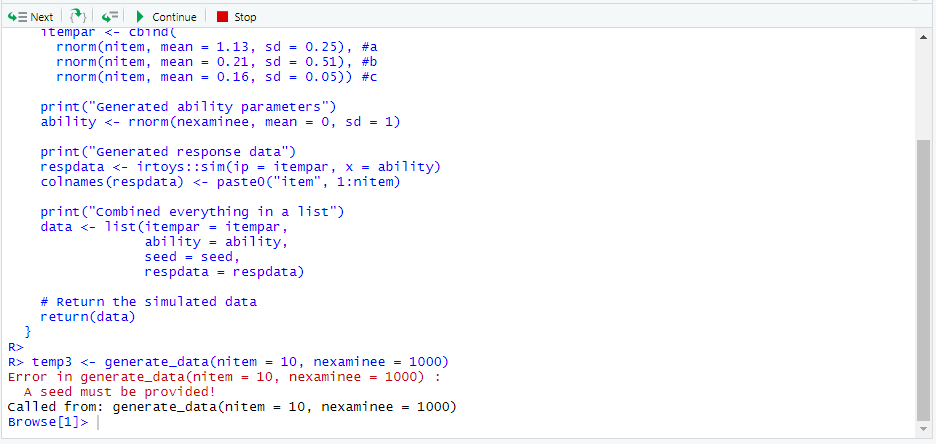
\includegraphics{figure/debug1.png}
\caption{Console once the interactive debugging begins}
\end{figure}

RStudio enables the browsing mode automatically in most cases -- this is why we have seen \texttt{Browse{[}1{]}\textgreater{}} after the error occured in the code. Using the browser buttons, we can evaluate the next statement, evaluate the next statement but step into the current function, execute the remainder of the function, continue executing the code until the next error or breaking point, or exit the debug mode, based on the buttons from left to right (see the figure below).

\begin{figure}
\centering
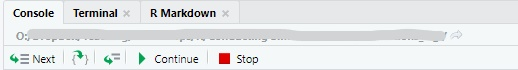
\includegraphics{figure/Inkeddebug3_LI.jpg}
\caption{Debugging menu options}
\end{figure}

In addition to the console, the source (where we are writing the codes) would show:

\begin{figure}
\centering
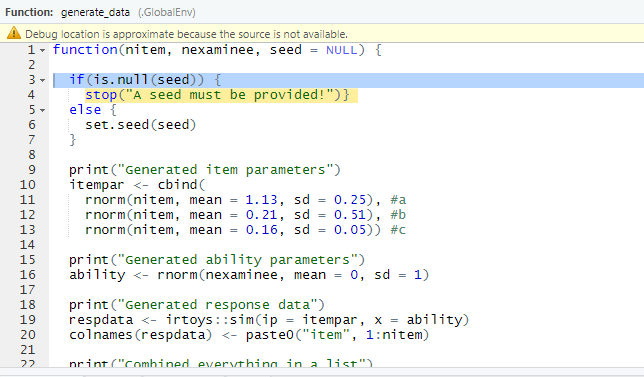
\includegraphics{figure/debug4.png}
\caption{Error location in the interactive debugging}
\end{figure}

The figure above shows that the browser was able to find the location of the error. We can also activate the debugging mode for a particular function using \texttt{debug()}. For example, using \texttt{debug(generate\_data)} and running \texttt{temp3\ \textless{}-\ generate\_data(nitem\ =\ 10,\ nexaminee\ =\ 1000)} will show the following output in the console. By clicking on the ``next'' button, we can debug the code slowly and see where the error occurred. Once we are satisfied with the function, we can turn off the interactive debugging mode using the \texttt{undebug()} function.

\begin{figure}
\centering
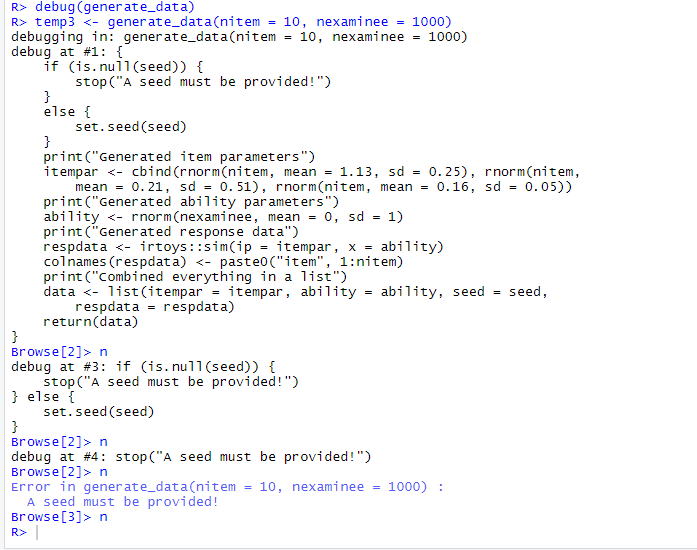
\includegraphics{figure/debug5.png}
\caption{Using the debug() function}
\end{figure}

If we want to see how we came to this particular error in the function, we can hit ``enter'' to exit the browser mode and type \texttt{traceback()}. This would return the steps that we have taken until the error message:

\begin{figure}
\centering
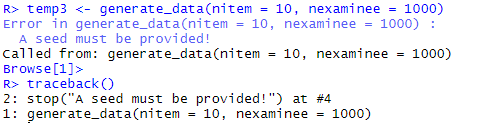
\includegraphics{figure/debug2.png}
\caption{The traceback() option in R}
\end{figure}

\begin{center}\rule{0.5\linewidth}{0.5pt}\end{center}

For more further information about debugging in \texttt{R}, I highly recommend you to check out:

\begin{itemize}
\tightlist
\item
  the \href{https://adv-r.hadley.nz/debugging.html}{Debugging} chapter in Hadley Wickham's \href{https://adv-r.hadley.nz/}{Advanced R}, and
\item
  the \href{https://rstats.wtf/debugging-r-code.html}{Debugging R Code} chapter in Jennifer Bryan and Jim Hester's \href{https://rstats.wtf/}{What They Forgot to Teach You About R}
\end{itemize}

\begin{center}\rule{0.5\linewidth}{0.5pt}\end{center}

\hypertarget{putting-the-functions-together}{%
\section{Putting the Functions Together}\label{putting-the-functions-together}}

As we put all the custom functions together, we must determine:

\begin{enumerate}
\def\labelenumi{\arabic{enumi}.}
\tightlist
\item
  whether we want to run each custom function separately or in a single wrapper function that simply calls all of our custom functions
\item
  how we want to replicate our custom functions:
\end{enumerate}

\begin{itemize}
\tightlist
\item
  the \texttt{replicate} function
\item
  the \texttt{apply} function collection
\item
  loops (with single cluster or parallel computing)
\end{itemize}

\hypertarget{avoding-loops}{%
\subsection{Avoding Loops}\label{avoding-loops}}

One of the easiest ways to repeat the same function without a loop is to use the \texttt{replicate} function in \texttt{R}. The way this function works is very simple. Let's take a look at its basic structure:

\begin{Shaded}
\begin{Highlighting}[]
\KeywordTok{replicate}\NormalTok{(}\OperatorTok{<}\NormalTok{number of replications}\OperatorTok{>}\NormalTok{, }\OperatorTok{<}\ControlFlowTok{function}\NormalTok{ to be replicated}\OperatorTok{>}\NormalTok{)}
\end{Highlighting}
\end{Shaded}

Using the \texttt{repeat} function, we can run the \texttt{generate\_data} function many times very quickly. For example, let's create 5 data sets (i.e., 5 replications):

\begin{Shaded}
\begin{Highlighting}[]
\NormalTok{nreps =}\StringTok{ }\NormalTok{5L}
\NormalTok{x <-}\StringTok{ }\KeywordTok{replicate}\NormalTok{(nreps, }\KeywordTok{generate_data}\NormalTok{(}\DataTypeTok{nitem =} \DecValTok{10}\NormalTok{, }\DataTypeTok{nexaminee =} \DecValTok{1000}\NormalTok{))}
\KeywordTok{head}\NormalTok{(x)}
\end{Highlighting}
\end{Shaded}

\begin{verbatim}
         [,1]          [,2]          [,3]          [,4]          [,5]         
itempar  Numeric,30    Numeric,30    Numeric,30    Numeric,30    Numeric,30   
ability  Numeric,1000  Numeric,1000  Numeric,1000  Numeric,1000  Numeric,1000 
seed     8022          3891          7049          811           6957         
respdata Numeric,10000 Numeric,10000 Numeric,10000 Numeric,10000 Numeric,10000
\end{verbatim}

This would return an array (i.e., vector) called \texttt{x} which would store our simulated data sets returned from \texttt{generate\_data}. To call a particular data set from this array (e.g., data set 1), we would use:

\begin{Shaded}
\begin{Highlighting}[]
\NormalTok{x[,}\DecValTok{1}\NormalTok{]}
\end{Highlighting}
\end{Shaded}

which would return all the components (i.e., item parameters, ability parameters, seed, and response data) from data set 1.

Another effective method to repeat a function several times without a loop is to use the \texttt{apply} function collection: \texttt{apply()}, \texttt{sapply()}, and \texttt{lapply()}. The purpose of these functions is primarily to avoid explicit uses of loops when repeating a particular task in \texttt{R}\footnote{See \href{https://www.guru99.com/r-apply-sapply-tapply.html}{the Guru99 website} for more information on these functions.}. Among these three functions, \texttt{sapply()} and \texttt{lapply()} are particularly useful in simulations because they can apply an existing function (e..g, mean, median, sd) or a custom function to each element of an object. The difference between \texttt{lapply()} and \texttt{sapply()} lies between the output they return. \texttt{lapply()} applies a function and returns a list as its output, whereas \texttt{sapply()} returns a vector as its output.

In the following example, we want to extract the true item parameters from each replication stored in \texttt{x}. This is the first element of the output returned from \texttt{generate\_data}. Therefore, we will use both \texttt{lapply} and \texttt{sapply} to select the first element of 5 replications stored in \texttt{x}.

\begin{Shaded}
\begin{Highlighting}[]
\CommentTok{# lapply - returning a list}
\KeywordTok{lapply}\NormalTok{(1L}\OperatorTok{:}\NormalTok{nreps, }\ControlFlowTok{function}\NormalTok{(i) x[,i][}\DecValTok{1}\NormalTok{])}
\end{Highlighting}
\end{Shaded}

\begin{verbatim}
[[1]]
[[1]]$itempar
        [,1]    [,2]    [,3]
 [1,] 1.1415 -0.3682 0.07736
 [2,] 1.3827  0.3420 0.24551
 [3,] 1.0107  0.4589 0.14046
 [4,] 0.9634  0.1928 0.10050
 [5,] 1.0133  0.7065 0.23558
 [6,] 0.9482  0.1607 0.16483
 [7,] 0.8283 -0.3466 0.11231
 [8,] 1.3640  0.3054 0.17842
 [9,] 0.5806  0.3969 0.16591
[10,] 1.8895  0.1825 0.12764


[[2]]
[[2]]$itempar
        [,1]      [,2]    [,3]
 [1,] 0.8686  0.211830 0.23417
 [2,] 1.0666 -0.647674 0.22204
 [3,] 1.3665 -0.179088 0.15410
 [4,] 0.8196  0.206515 0.19359
 [5,] 1.2334  0.005374 0.25132
 [6,] 1.0186 -0.120199 0.27701
 [7,] 1.0917 -0.096444 0.20174
 [8,] 1.1214  0.387298 0.06626
 [9,] 1.4620 -0.353471 0.18427
[10,] 0.9542 -0.386885 0.11406


[[3]]
[[3]]$itempar
        [,1]      [,2]    [,3]
 [1,] 0.8242  0.596302 0.07725
 [2,] 1.6065 -0.290621 0.17878
 [3,] 1.2838  0.728311 0.20805
 [4,] 1.0859 -0.440566 0.16173
 [5,] 1.1749 -0.045554 0.23987
 [6,] 1.1786  0.006729 0.22537
 [7,] 0.8680  1.019832 0.15020
 [8,] 1.4489 -0.435660 0.14789
 [9,] 1.4630  1.346885 0.12883
[10,] 0.5805 -0.130311 0.26612


[[4]]
[[4]]$itempar
        [,1]     [,2]    [,3]
 [1,] 1.0833 -0.62881 0.18135
 [2,] 1.4569  0.35718 0.16981
 [3,] 1.4572  0.58300 0.15132
 [4,] 0.8332  0.77767 0.19911
 [5,] 0.7998  0.84951 0.07186
 [6,] 1.2964  1.40714 0.19965
 [7,] 1.0498  0.25638 0.23851
 [8,] 1.1080 -0.58124 0.16927
 [9,] 0.7451  0.08085 0.18025
[10,] 0.8302  0.61757 0.18997


[[5]]
[[5]]$itempar
        [,1]     [,2]    [,3]
 [1,] 1.2428  0.38038 0.15683
 [2,] 0.9222  0.06897 0.14285
 [3,] 1.2159 -0.53983 0.08549
 [4,] 1.3092  0.47354 0.17746
 [5,] 1.0709 -0.15980 0.20135
 [6,] 0.8401  0.70899 0.20493
 [7,] 1.0457 -0.57915 0.19977
 [8,] 1.0311  0.96456 0.22195
 [9,] 1.4022 -0.48486 0.16690
[10,] 0.8243 -0.12529 0.11996
\end{verbatim}

\begin{Shaded}
\begin{Highlighting}[]
\CommentTok{# sapply - returning a vector or matrix}
\KeywordTok{sapply}\NormalTok{(1L}\OperatorTok{:}\NormalTok{nreps, }\ControlFlowTok{function}\NormalTok{(i) x[,i][}\DecValTok{1}\NormalTok{])}
\end{Highlighting}
\end{Shaded}

\begin{verbatim}
$itempar
        [,1]    [,2]    [,3]
 [1,] 1.1415 -0.3682 0.07736
 [2,] 1.3827  0.3420 0.24551
 [3,] 1.0107  0.4589 0.14046
 [4,] 0.9634  0.1928 0.10050
 [5,] 1.0133  0.7065 0.23558
 [6,] 0.9482  0.1607 0.16483
 [7,] 0.8283 -0.3466 0.11231
 [8,] 1.3640  0.3054 0.17842
 [9,] 0.5806  0.3969 0.16591
[10,] 1.8895  0.1825 0.12764

$itempar
        [,1]      [,2]    [,3]
 [1,] 0.8686  0.211830 0.23417
 [2,] 1.0666 -0.647674 0.22204
 [3,] 1.3665 -0.179088 0.15410
 [4,] 0.8196  0.206515 0.19359
 [5,] 1.2334  0.005374 0.25132
 [6,] 1.0186 -0.120199 0.27701
 [7,] 1.0917 -0.096444 0.20174
 [8,] 1.1214  0.387298 0.06626
 [9,] 1.4620 -0.353471 0.18427
[10,] 0.9542 -0.386885 0.11406

$itempar
        [,1]      [,2]    [,3]
 [1,] 0.8242  0.596302 0.07725
 [2,] 1.6065 -0.290621 0.17878
 [3,] 1.2838  0.728311 0.20805
 [4,] 1.0859 -0.440566 0.16173
 [5,] 1.1749 -0.045554 0.23987
 [6,] 1.1786  0.006729 0.22537
 [7,] 0.8680  1.019832 0.15020
 [8,] 1.4489 -0.435660 0.14789
 [9,] 1.4630  1.346885 0.12883
[10,] 0.5805 -0.130311 0.26612

$itempar
        [,1]     [,2]    [,3]
 [1,] 1.0833 -0.62881 0.18135
 [2,] 1.4569  0.35718 0.16981
 [3,] 1.4572  0.58300 0.15132
 [4,] 0.8332  0.77767 0.19911
 [5,] 0.7998  0.84951 0.07186
 [6,] 1.2964  1.40714 0.19965
 [7,] 1.0498  0.25638 0.23851
 [8,] 1.1080 -0.58124 0.16927
 [9,] 0.7451  0.08085 0.18025
[10,] 0.8302  0.61757 0.18997

$itempar
        [,1]     [,2]    [,3]
 [1,] 1.2428  0.38038 0.15683
 [2,] 0.9222  0.06897 0.14285
 [3,] 1.2159 -0.53983 0.08549
 [4,] 1.3092  0.47354 0.17746
 [5,] 1.0709 -0.15980 0.20135
 [6,] 0.8401  0.70899 0.20493
 [7,] 1.0457 -0.57915 0.19977
 [8,] 1.0311  0.96456 0.22195
 [9,] 1.4022 -0.48486 0.16690
[10,] 0.8243 -0.12529 0.11996
\end{verbatim}

This is a very simple example of how \texttt{lapply} and \texttt{sapply} work. Using the same structure, we could also estimate the item parameters with \texttt{mirt} and save all the results together.

\begin{Shaded}
\begin{Highlighting}[]
\NormalTok{data <-}\StringTok{ }\KeywordTok{lapply}\NormalTok{(1L}\OperatorTok{:}\NormalTok{nreps, }
               \ControlFlowTok{function}\NormalTok{(i) x[,i][}\DecValTok{4}\NormalTok{]) }\CommentTok{# the 4th part is respdata}

\NormalTok{models <-}\StringTok{ }\KeywordTok{lapply}\NormalTok{(}\KeywordTok{lapply}\NormalTok{(data, }\StringTok{'[['}\NormalTok{, }\StringTok{'respdata'}\NormalTok{), }\CommentTok{# select respdata from each list}
                 \ControlFlowTok{function}\NormalTok{(i) mirt}\OperatorTok{::}\KeywordTok{mirt}\NormalTok{(}\DataTypeTok{data =}\NormalTok{ i, }\DecValTok{1}\NormalTok{, }\DataTypeTok{itemtype =} \StringTok{"3PL"}\NormalTok{)) }\CommentTok{# apply mirt to respdata}

\NormalTok{parameters <-}\StringTok{ }\KeywordTok{lapply}\NormalTok{(models, }
                     \ControlFlowTok{function}\NormalTok{(x) mirt}\OperatorTok{::}\KeywordTok{coef}\NormalTok{(x, }\DataTypeTok{IRTpars =} \OtherTok{TRUE}\NormalTok{, }\DataTypeTok{simplify =} \OtherTok{TRUE}\NormalTok{)}\OperatorTok{$}\NormalTok{items[,}\DecValTok{1}\OperatorTok{:}\DecValTok{3}\NormalTok{])}
\end{Highlighting}
\end{Shaded}

\hypertarget{loops}{%
\subsection{Loops}\label{loops}}

Loops in \texttt{R} are useful when:

\begin{itemize}
\tightlist
\item
  there is a series of functions to be executed and
\item
  the functions return a particular object (e.g., an integer, a data frame, or a matrix) that is necessary for the subsequent functions.
\end{itemize}

There are several control statements essential for loops:

\begin{itemize}
\tightlist
\item
  \texttt{if} and \texttt{else} for testing a condition and acting on it
\item
  \texttt{for} for setting up and running a loop a fixed number of iterations
\item
  \texttt{while} for executing a loop while a condition is true
\item
  \texttt{break} for stopping the execution of a loop
\item
  \texttt{next} for skipping an iteration of a loop
\end{itemize}

Let's take a quick look at how each of these control statements works:

\textbf{if-else statement}

\begin{Shaded}
\begin{Highlighting}[]
\ControlFlowTok{if}\NormalTok{(}\OperatorTok{<}\NormalTok{condition1}\OperatorTok{>}\NormalTok{) \{}
  \CommentTok{## do action #1}
\NormalTok{  \} }\ControlFlowTok{else} \ControlFlowTok{if}\NormalTok{(}\OperatorTok{<}\NormalTok{condition2}\OperatorTok{>}\NormalTok{)  \{}
    \CommentTok{## do action #2}
\NormalTok{    \} }\ControlFlowTok{else}\NormalTok{ \{}
      \CommentTok{## do action #3}
\NormalTok{      \}}
\end{Highlighting}
\end{Shaded}

\textbf{for statement}

\begin{Shaded}
\begin{Highlighting}[]
\ControlFlowTok{for}\NormalTok{(}\OperatorTok{<}\NormalTok{index1}\OperatorTok{>}\StringTok{ }\ControlFlowTok{in} \OperatorTok{<}\NormalTok{values of index1}\OperatorTok{>}\NormalTok{) \{}
  \ControlFlowTok{for}\NormalTok{(}\OperatorTok{<}\NormalTok{index2}\OperatorTok{>}\StringTok{ }\ControlFlowTok{in} \OperatorTok{<}\NormalTok{values of index2}\OperatorTok{>}\NormalTok{) \{}
    \CommentTok{## do an action for each index1 and index2}
\NormalTok{  \}}
\NormalTok{\}}
\end{Highlighting}
\end{Shaded}

\textbf{while statement}

\begin{Shaded}
\begin{Highlighting}[]
\ControlFlowTok{while}\NormalTok{(}\OperatorTok{<}\NormalTok{condition}\OperatorTok{>}\NormalTok{) \{}
  \CommentTok{## do an action while condition == TRUE}
\NormalTok{\}}
\end{Highlighting}
\end{Shaded}

\textbf{break statement}

\begin{Shaded}
\begin{Highlighting}[]
\ControlFlowTok{for}\NormalTok{(}\OperatorTok{<}\NormalTok{index}\OperatorTok{>}\StringTok{ }\ControlFlowTok{in} \OperatorTok{<}\NormalTok{values of index}\OperatorTok{>}\NormalTok{) \{}
  \CommentTok{## do an action for each index}
  \ControlFlowTok{if}\NormalTok{(}\OperatorTok{<}\NormalTok{condition}\OperatorTok{>}\NormalTok{) \{}
    \ControlFlowTok{break} \CommentTok{# Stop the action if condition == TRUE}
\NormalTok{  \}}
\NormalTok{\}}
\end{Highlighting}
\end{Shaded}

\textbf{next statement}

\begin{Shaded}
\begin{Highlighting}[]
\ControlFlowTok{for}\NormalTok{(}\OperatorTok{<}\NormalTok{index}\OperatorTok{>}\StringTok{ }\ControlFlowTok{in} \OperatorTok{<}\NormalTok{values of index}\OperatorTok{>}\NormalTok{) \{}
  \ControlFlowTok{if}\NormalTok{(}\OperatorTok{<}\NormalTok{condition}\OperatorTok{>}\NormalTok{) \{}
    \ControlFlowTok{next} \CommentTok{## Skip the action if condition == TRUE}
\NormalTok{  \}}
  \CommentTok{## do an action for each index}
\NormalTok{\}}
\end{Highlighting}
\end{Shaded}

In general, loops are very useful in Monte Carlo simulations; however, they can be very slow when:

\begin{itemize}
\tightlist
\item
  we are dealing with heavy computations
\item
  we apply a function to each row or column of a large data set
\end{itemize}

Therefore, compared with traditional \texttt{for} loops, the \texttt{apply} function collection is often more preferable because it can run a computation and return its results much more quickly.

\hypertarget{parallel-computing}{%
\subsection{Parallel Computing}\label{parallel-computing}}

In some computations, creating a loop might be necessary. The regular \texttt{for} loop statement executes all the functions using a single processor in the computer. Similarly, the \texttt{apply} function collection also utilizes a single processor in the computer. The use of a single processor is the default setting in \texttt{R}. That is, regardless of whether we are using a 64-bit version of \texttt{R} in a multi-core, powerful computer, \texttt{R} always uses only \textbf{one} processor by default.

For example, in a simulation study with 100 replications via \texttt{for} loops, a single processor would have to run each iteration one by one and return the results once all replications are completed. This may not be a problem especially if we are running a very simple simulation. However, completing a simulation study involving heavy computations for each replication, using a single processor could be very time consuming. Fortunately, there is a solution to this problem: \textbf{parallel computing}\footnote{For a quick introduction to parallel computing in \texttt{R}, you can check out \href{https://nceas.github.io/oss-lessons/parallel-computing-in-r/parallel-computing-in-r.html}{this website}.}.

To benefit from parallel computing when running a Monte Carlo simulation study, we will use two packages: \texttt{foreach} \citep{R-foreach} and \texttt{doParallel} \citep{R-doParallel}. \texttt{doParallel} essentially provides a mechanism
needed to execute \texttt{foreach} loops in parallel computing (see the \href{https://cran.r-project.org/web/packages/doParallel/vignettes/gettingstartedParallel.pdf}{vignette} for the \texttt{doParallel} package).

There are several steps in setting up parallel computing with \texttt{doParallel}:

\begin{enumerate}
\def\labelenumi{\arabic{enumi}.}
\tightlist
\item
  Make clusters for parallel computing
\item
  Register clusters with \texttt{doParallel}
\item
  Run \texttt{foreach} loops using parallel computing.
\end{enumerate}

Now, let's take a look at a short example. First, we will activate \texttt{doParallel}. Next, we will check how many processors (i.e., cores) are available in our computer. The number of processors is the maximum number that we can use when setting up parallel computing. This would use all the processors available, though it also slows down the computer significantly and prevents us from doing other tasks in the computer. If this is a concern, then we can assign fewer processors (instead of all of them) to parallel computing.

\begin{Shaded}
\begin{Highlighting}[]
\KeywordTok{library}\NormalTok{(}\StringTok{"doParallel"}\NormalTok{)}
\KeywordTok{detectCores}\NormalTok{()}
\end{Highlighting}
\end{Shaded}

\begin{verbatim}
[1] 16
\end{verbatim}

It seems that there are 16 processors available. We want to use 4 of these processors for running parallel loops\footnote{If the computer has a Mac operating system, then \texttt{cl\ \textless{}-\ makeCluster(4,\ outfile="")} should be used.}.

\begin{Shaded}
\begin{Highlighting}[]
\NormalTok{cl <-}\StringTok{ }\KeywordTok{makeCluster}\NormalTok{(}\DecValTok{4}\NormalTok{) }\CommentTok{# Register four clusters (Windows)}
\KeywordTok{registerDoParallel}\NormalTok{(cl)}
\end{Highlighting}
\end{Shaded}

In a \texttt{foreach} loop, there are two ways that a loop can be set up: \texttt{\%do\%} for a regular loop and \texttt{\%dopar\%} for running the same code sequentially through multiple processors. In the following example, we will use \texttt{\%dopar\%}.

\begin{Shaded}
\begin{Highlighting}[]
\KeywordTok{foreach}\NormalTok{(}\DataTypeTok{i=}\DecValTok{1}\OperatorTok{:}\DecValTok{4}\NormalTok{) }\OperatorTok\StringTok{ }\KeywordTok{sqrt}\NormalTok{(i)}
\KeywordTok{stopCluster}\NormalTok{(cl) }\CommentTok{# Stop using clusters}
\end{Highlighting}
\end{Shaded}

Once the simulation is over, we will turn off the clusters.

\begin{Shaded}
\begin{Highlighting}[]
\KeywordTok{stopCluster}\NormalTok{(cl) }\CommentTok{# Stop using clusters}
\end{Highlighting}
\end{Shaded}

In this small example, it is hard to see the impact of parallel computing. Parallel computing will show its strengths more clearly when we check the computing time (i.e., running time) of our codes. We will talk about this in the next section.

To demonstrate how to put all the simulation functions together, we will combine the custom functions and run them together within a loop. First, we will run the latest (i.e., tested) versions of our custom functions:

\begin{Shaded}
\begin{Highlighting}[]
\CommentTok{# Function #1}
\NormalTok{generate_data <-}\StringTok{ }\ControlFlowTok{function}\NormalTok{(nitem, nexaminee, }\DataTypeTok{seed =} \OtherTok{NULL}\NormalTok{) \{}
  
  \ControlFlowTok{if}\NormalTok{(}\OperatorTok{!}\KeywordTok{is.null}\NormalTok{(seed)) \{}
    \KeywordTok{set.seed}\NormalTok{(seed)\} }
  \ControlFlowTok{else}\NormalTok{ \{}
    \KeywordTok{warning}\NormalTok{(}\StringTok{"No seed provided!"}\NormalTok{, }\DataTypeTok{call. =} \OtherTok{FALSE}\NormalTok{)}
\NormalTok{    seed <-}\StringTok{ }\KeywordTok{sample.int}\NormalTok{(}\DecValTok{10000}\NormalTok{, }\DecValTok{1}\NormalTok{)}
    \KeywordTok{set.seed}\NormalTok{(seed)}
    \KeywordTok{message}\NormalTok{(}\StringTok{"Random seed = "}\NormalTok{, seed, }\StringTok{"}\CharTok{\textbackslash{}n}\StringTok{"}\NormalTok{)}
\NormalTok{  \}}
  
\NormalTok{  itempar <-}\StringTok{ }\KeywordTok{cbind}\NormalTok{(}
    \KeywordTok{rnorm}\NormalTok{(nitem, }\DataTypeTok{mean =} \FloatTok{1.13}\NormalTok{, }\DataTypeTok{sd =} \FloatTok{0.25}\NormalTok{), }\CommentTok{#a}
    \KeywordTok{rnorm}\NormalTok{(nitem, }\DataTypeTok{mean =} \FloatTok{0.21}\NormalTok{, }\DataTypeTok{sd =} \FloatTok{0.51}\NormalTok{), }\CommentTok{#b}
    \KeywordTok{rnorm}\NormalTok{(nitem, }\DataTypeTok{mean =} \FloatTok{0.16}\NormalTok{, }\DataTypeTok{sd =} \FloatTok{0.05}\NormalTok{)) }\CommentTok{#c}
  
\NormalTok{  ability <-}\StringTok{ }\KeywordTok{rnorm}\NormalTok{(nexaminee, }\DataTypeTok{mean =} \DecValTok{0}\NormalTok{, }\DataTypeTok{sd =} \DecValTok{1}\NormalTok{)}
  
\NormalTok{  respdata <-}\StringTok{ }\NormalTok{irtoys}\OperatorTok{::}\KeywordTok{sim}\NormalTok{(}\DataTypeTok{ip =}\NormalTok{ itempar, }\DataTypeTok{x =}\NormalTok{ ability)}
  \KeywordTok{colnames}\NormalTok{(respdata) <-}\StringTok{ }\KeywordTok{paste0}\NormalTok{(}\StringTok{"item"}\NormalTok{, }\DecValTok{1}\OperatorTok{:}\NormalTok{nitem)}
  
\NormalTok{  data <-}\StringTok{ }\KeywordTok{list}\NormalTok{(}\DataTypeTok{itempar =}\NormalTok{ itempar,}
               \DataTypeTok{ability =}\NormalTok{ ability,}
               \DataTypeTok{seed =}\NormalTok{ seed,}
               \DataTypeTok{respdata =}\NormalTok{ respdata)}
  
  \KeywordTok{return}\NormalTok{(data)}
\NormalTok{\}}

\CommentTok{# Function 2}
\NormalTok{estimate_par <-}\StringTok{ }\ControlFlowTok{function}\NormalTok{(data, }\DataTypeTok{guess =} \DecValTok{-1}\NormalTok{) \{}
  \CommentTok{# If guessing is fixed}
  \ControlFlowTok{if}\NormalTok{(guess }\OperatorTok{>=}\StringTok{ }\DecValTok{0}\NormalTok{) \{}
    
    \CommentTok{# Model set up}
\NormalTok{    mod3PL <-}\StringTok{ }\NormalTok{mirt}\OperatorTok{::}\KeywordTok{mirt}\NormalTok{(data, }\CommentTok{# response data}
                         \DecValTok{1}\NormalTok{,    }\CommentTok{# unidimensional model}
                         \DataTypeTok{guess =}\NormalTok{ guess, }\CommentTok{# fixed guessing}
                         \DataTypeTok{verbose =} \OtherTok{FALSE}\NormalTok{, }\CommentTok{# Don't print verbose}
                         \CommentTok{# Increase the number of EM cycles}
                         \CommentTok{# Turn off estimation messages}
                         \DataTypeTok{technical =} \KeywordTok{list}\NormalTok{(}\DataTypeTok{NCYCLES =} \DecValTok{1000}\NormalTok{,}
                                          \DataTypeTok{message =} \OtherTok{FALSE}\NormalTok{)) }
\NormalTok{  \} }\ControlFlowTok{else}\NormalTok{ \{}
\NormalTok{    mod3PL <-}\StringTok{ }\NormalTok{mirt}\OperatorTok{::}\KeywordTok{mirt}\NormalTok{(data, }\CommentTok{# response data}
                         \DecValTok{1}\NormalTok{,    }\CommentTok{# unidimensional model}
                         \DataTypeTok{itemtype =} \StringTok{"3PL"}\NormalTok{, }\CommentTok{# IRT model}
                         \DataTypeTok{verbose =} \OtherTok{FALSE}\NormalTok{, }\CommentTok{# Don't print verbose}
                         \CommentTok{# Increase the number of EM cycles}
                         \CommentTok{# Turn off estimation messages}
                         \DataTypeTok{technical =} \KeywordTok{list}\NormalTok{(}\DataTypeTok{NCYCLES =} \DecValTok{1000}\NormalTok{,}
                                          \DataTypeTok{message =} \OtherTok{FALSE}\NormalTok{)) }
\NormalTok{  \}}
  
  \CommentTok{# Extract item parameters in typical IRT metric}
\NormalTok{  itempar_est <-}\StringTok{ }\KeywordTok{as.data.frame}\NormalTok{(mirt}\OperatorTok{::}\KeywordTok{coef}\NormalTok{(mod3PL, }\DataTypeTok{IRTpars =} \OtherTok{TRUE}\NormalTok{, }\DataTypeTok{simplify =} \OtherTok{TRUE}\NormalTok{)}\OperatorTok{$}\NormalTok{item[,}\DecValTok{1}\OperatorTok{:}\DecValTok{3}\NormalTok{])}
  \KeywordTok{return}\NormalTok{(itempar_est)}
\NormalTok{\}}

\CommentTok{# Function #3}
\NormalTok{summarize <-}\StringTok{ }\ControlFlowTok{function}\NormalTok{(est_params, true_params) \{}
\NormalTok{  result <-}\StringTok{ }\KeywordTok{data.frame}\NormalTok{(}
    \DataTypeTok{parameter =} \KeywordTok{c}\NormalTok{(}\StringTok{"a"}\NormalTok{, }\StringTok{"b"}\NormalTok{, }\StringTok{"c"}\NormalTok{),}
    \DataTypeTok{bias =} \KeywordTok{sapply}\NormalTok{(1L}\OperatorTok{:}\NormalTok{3L, }\ControlFlowTok{function}\NormalTok{(i) }\KeywordTok{mean}\NormalTok{((est_params[, i] }\OperatorTok{-}\StringTok{ }\NormalTok{true_params[,i]))),}
    \DataTypeTok{rmse =} \KeywordTok{sapply}\NormalTok{(1L}\OperatorTok{:}\NormalTok{3L, }\ControlFlowTok{function}\NormalTok{(i) }\KeywordTok{sqrt}\NormalTok{(}\KeywordTok{mean}\NormalTok{((est_params[, i] }\OperatorTok{-}\StringTok{ }\NormalTok{true_params[,i])}\OperatorTok{^}\DecValTok{2}\NormalTok{))),}
    \DataTypeTok{correlation =} \KeywordTok{sapply}\NormalTok{(1L}\OperatorTok{:}\NormalTok{3L, }\ControlFlowTok{function}\NormalTok{(i) }\KeywordTok{cor}\NormalTok{(est_params[, i], true_params[,i])))}
  \KeywordTok{return}\NormalTok{(result)}
\NormalTok{\}}
\end{Highlighting}
\end{Shaded}

Second, we will set up our simulation conditions so that it would be easier to update them as we run all the conditions. Note that the number of iterations (i.e., replications) is only 4 for now. If the functions work as expected, we will increase the number of iterations to 100.

\begin{Shaded}
\begin{Highlighting}[]
\NormalTok{iterations =}\StringTok{ }\DecValTok{4} \CommentTok{# Only 4 iteration for now}
\NormalTok{seed =}\StringTok{ }\KeywordTok{sample.int}\NormalTok{(}\DecValTok{10000}\NormalTok{, }\DecValTok{100}\NormalTok{)}
\NormalTok{nitem =}\StringTok{ }\DecValTok{10} \CommentTok{# 10, 15, 20, or 25}
\NormalTok{nexaminee =}\StringTok{ }\DecValTok{1000} \CommentTok{# 250, 500, 750, or 1000}
\NormalTok{guess =}\StringTok{ }\DecValTok{-1} \CommentTok{# A negative value or a value from 0 to 1}
\end{Highlighting}
\end{Shaded}

Third, we will set up parallel computing and register multiple processors for the simulation.

\begin{Shaded}
\begin{Highlighting}[]
\NormalTok{cl <-}\StringTok{ }\KeywordTok{makeCluster}\NormalTok{(}\DecValTok{4}\NormalTok{) }\CommentTok{# Register four clusters}
\KeywordTok{registerDoParallel}\NormalTok{(cl)}
\end{Highlighting}
\end{Shaded}

Finally, we will run our simulation and save the results as \texttt{simresults}.

\begin{Shaded}
\begin{Highlighting}[]
\NormalTok{simresults <-}\StringTok{ }\KeywordTok{foreach}\NormalTok{(}\DataTypeTok{i=}\DecValTok{1}\OperatorTok{:}\NormalTok{iterations, }
                      \DataTypeTok{.packages =} \KeywordTok{c}\NormalTok{(}\StringTok{"mirt"}\NormalTok{, }\StringTok{"doParallel"}\NormalTok{),}
                      \DataTypeTok{.combine =}\NormalTok{ rbind) }\OperatorTok\StringTok{ }\NormalTok{\{}
                        \CommentTok{# Generate item parameters and data}
\NormalTok{                        step1 <-}\StringTok{ }\KeywordTok{generate_data}\NormalTok{(}\DataTypeTok{nitem=}\NormalTok{nitem, }\DataTypeTok{nexaminee=}\NormalTok{nexaminee, }\DataTypeTok{seed=}\NormalTok{seed[i])}
                        \CommentTok{# Estimate item parameters}
\NormalTok{                        step2 <-}\StringTok{ }\KeywordTok{estimate_par}\NormalTok{(step1}\OperatorTok{$}\NormalTok{respdata, }\DataTypeTok{guess =}\NormalTok{ guess)}
                        \CommentTok{# Summarize results}
                        \KeywordTok{summarize}\NormalTok{(step2, step1}\OperatorTok{$}\NormalTok{itempar)}
\NormalTok{                        \} }
\end{Highlighting}
\end{Shaded}

Now, we can see the results (assuming no error messages appeared on our console):

\begin{Shaded}
\begin{Highlighting}[]
\NormalTok{simresults}
\end{Highlighting}
\end{Shaded}

\begin{verbatim}
   parameter      bias   rmse correlation
1          a  0.128163 0.3748     0.78904
2          b -0.059314 0.5941     0.62520
3          c -0.025765 0.1377     0.24511
4          a -0.030007 0.3135     0.49103
5          b -0.244383 0.4692     0.88362
6          c -0.052045 0.1444    -0.27393
7          a  0.199876 0.7391    -0.08689
8          b  0.017008 0.2874     0.82013
9          c  0.002217 0.1187     0.13883
10         a  0.310501 0.4886     0.78836
11         b  0.129384 0.3310     0.84102
12         c  0.072968 0.1203     0.42944
\end{verbatim}

Remember that this is only for \textbf{one} of the crossed conditions (10 items, 1000 examinees, no fixed guessing) across \textbf{four} iterations. We can summarize the results across all iterations, add additional information to remind us what we have done in the simulation, and save the results. We will use the \texttt{dplyr} package \citep{R-dplyr} for summarizing our simulation results.

\begin{Shaded}
\begin{Highlighting}[]
\KeywordTok{library}\NormalTok{(}\StringTok{"dplyr"}\NormalTok{)}

\NormalTok{simresults_final <-}\StringTok{ }\NormalTok{simresults }\OperatorTok
\StringTok{  }\KeywordTok{group_by}\NormalTok{(parameter) }\OperatorTok
\StringTok{  }\CommentTok{# Find the average and rounded values }
\StringTok{  }\KeywordTok{summarise}\NormalTok{(}\DataTypeTok{bias =} \KeywordTok{round}\NormalTok{(}\KeywordTok{mean}\NormalTok{(bias),}\DecValTok{3}\NormalTok{),}
            \DataTypeTok{rmse =} \KeywordTok{round}\NormalTok{(}\KeywordTok{mean}\NormalTok{(rmse),}\DecValTok{3}\NormalTok{),}
            \DataTypeTok{correlation =} \KeywordTok{round}\NormalTok{(}\KeywordTok{mean}\NormalTok{(correlation),}\DecValTok{3}\NormalTok{)) }\OperatorTok
\StringTok{  }\KeywordTok{mutate}\NormalTok{(}\DataTypeTok{nitem =}\NormalTok{ nitem,}
         \DataTypeTok{nexaminee =}\NormalTok{ nexaminee,}
         \DataTypeTok{guess =}\NormalTok{ guess) }\OperatorTok
\StringTok{  }\KeywordTok{select}\NormalTok{(nitem, nexaminee, guess, parameter, bias, rmse, correlation) }\OperatorTok
\StringTok{  }\KeywordTok{as.data.frame}\NormalTok{()}

\NormalTok{simresults_final}
\end{Highlighting}
\end{Shaded}

\begin{verbatim}
  nitem nexaminee guess parameter   bias  rmse correlation
1    10      1000    -1         a  0.152 0.479       0.495
2    10      1000    -1         b -0.039 0.420       0.792
3    10      1000    -1         c -0.001 0.130       0.135
\end{verbatim}

We can also create a nested loop where we can all the conditions together. Here we use \texttt{\%:\%} to set up three nested loops without curly brackets. The final loop contains \texttt{\%dopar\%} with curly brackets and closes all the loops. Note that we included the final summary function (see how \texttt{step3} is summarized) inside these nested loops. This will return a long-format summary data set with all the conditions based on \textbf{100} iterations.

\begin{Shaded}
\begin{Highlighting}[]
\CommentTok{# Set all the conditions}
\NormalTok{iterations =}\StringTok{ }\DecValTok{100}
\NormalTok{seed =}\StringTok{ }\KeywordTok{sample.int}\NormalTok{(}\DecValTok{10000}\NormalTok{, }\DecValTok{100}\NormalTok{)}
\NormalTok{nitem =}\StringTok{ }\KeywordTok{c}\NormalTok{(}\DecValTok{10}\NormalTok{, }\DecValTok{15}\NormalTok{, }\DecValTok{20}\NormalTok{, }\DecValTok{25}\NormalTok{)}
\NormalTok{nexaminee =}\StringTok{ }\KeywordTok{c}\NormalTok{(}\DecValTok{250}\NormalTok{, }\DecValTok{500}\NormalTok{, }\DecValTok{750}\NormalTok{, }\DecValTok{1000}\NormalTok{)}
\NormalTok{guess =}\StringTok{ }\KeywordTok{c}\NormalTok{(}\OperatorTok{-}\DecValTok{1}\NormalTok{, }\FloatTok{0.16}\NormalTok{)}

\CommentTok{# Register four clusters}
\NormalTok{cl <-}\StringTok{ }\KeywordTok{makeCluster}\NormalTok{(}\DecValTok{4}\NormalTok{) }
\KeywordTok{registerDoParallel}\NormalTok{(cl)}

\CommentTok{# Run nested foreach loops}
\NormalTok{simresults <-}\StringTok{ }\KeywordTok{foreach}\NormalTok{(}\DataTypeTok{i=}\DecValTok{1}\OperatorTok{:}\NormalTok{iterations, }
                      \DataTypeTok{.packages =} \KeywordTok{c}\NormalTok{(}\StringTok{"mirt"}\NormalTok{, }\StringTok{"doParallel"}\NormalTok{, }\StringTok{"dplyr"}\NormalTok{),}
                      \DataTypeTok{.combine =}\NormalTok{ rbind) }\OperatorTok
\StringTok{  }\KeywordTok{foreach}\NormalTok{(}\DataTypeTok{j=}\NormalTok{nitem, }
          \DataTypeTok{.packages =} \KeywordTok{c}\NormalTok{(}\StringTok{"mirt"}\NormalTok{, }\StringTok{"doParallel"}\NormalTok{, }\StringTok{"dplyr"}\NormalTok{),}
          \DataTypeTok{.combine =}\NormalTok{ rbind)  }\OperatorTok
\StringTok{  }
\StringTok{ }\KeywordTok{foreach}\NormalTok{(}\DataTypeTok{k=}\NormalTok{nexaminee, }
          \DataTypeTok{.packages =} \KeywordTok{c}\NormalTok{(}\StringTok{"mirt"}\NormalTok{, }\StringTok{"doParallel"}\NormalTok{, }\StringTok{"dplyr"}\NormalTok{),}
          \DataTypeTok{.combine =}\NormalTok{ rbind)  }\OperatorTok
\StringTok{  }
\StringTok{  }\KeywordTok{foreach}\NormalTok{(}\DataTypeTok{m=}\NormalTok{guess, }
          \DataTypeTok{.packages =} \KeywordTok{c}\NormalTok{(}\StringTok{"mirt"}\NormalTok{, }\StringTok{"doParallel"}\NormalTok{, }\StringTok{"dplyr"}\NormalTok{),}
          \DataTypeTok{.combine =}\NormalTok{ rbind)  }\OperatorTok\StringTok{ }\NormalTok{\{}
            \CommentTok{# Generate item parameters and data}
\NormalTok{            step1 <-}\StringTok{ }\KeywordTok{generate_data}\NormalTok{(}\DataTypeTok{nitem=}\NormalTok{j, }\DataTypeTok{nexaminee=}\NormalTok{k, }\DataTypeTok{seed=}\NormalTok{seed[i])}
            \CommentTok{# Estimate item parameters}
\NormalTok{            step2 <-}\StringTok{ }\KeywordTok{estimate_par}\NormalTok{(step1}\OperatorTok{$}\NormalTok{respdata, }\DataTypeTok{guess =}\NormalTok{ m)}
            \CommentTok{# Summarize results}
\NormalTok{            step3 <-}\StringTok{ }\KeywordTok{summarize}\NormalTok{(step2, step1}\OperatorTok{$}\NormalTok{itempar)}
            \CommentTok{# Finalize results}
\NormalTok{            step3 }\OperatorTok
\StringTok{              }\KeywordTok{group_by}\NormalTok{(parameter) }\OperatorTok
\StringTok{              }\KeywordTok{summarise}\NormalTok{(}\DataTypeTok{bias =} \KeywordTok{round}\NormalTok{(}\KeywordTok{mean}\NormalTok{(bias),}\DecValTok{3}\NormalTok{),}
                        \DataTypeTok{rmse =} \KeywordTok{round}\NormalTok{(}\KeywordTok{mean}\NormalTok{(rmse),}\DecValTok{3}\NormalTok{),}
                        \DataTypeTok{correlation =} \KeywordTok{round}\NormalTok{(}\KeywordTok{mean}\NormalTok{(correlation),}\DecValTok{3}\NormalTok{)) }\OperatorTok
\StringTok{              }\KeywordTok{mutate}\NormalTok{(}\DataTypeTok{nitem =}\NormalTok{ j,}
                     \DataTypeTok{nexaminee =}\NormalTok{ k,}
                     \DataTypeTok{guess =}\NormalTok{ m) }\OperatorTok
\StringTok{              }\KeywordTok{select}\NormalTok{(nitem, nexaminee, guess, parameter, bias, rmse, correlation) }\OperatorTok
\StringTok{              }\KeywordTok{as.data.frame}\NormalTok{()}
\NormalTok{          \}}

\CommentTok{# Stop the clusters}
\KeywordTok{stopCluster}\NormalTok{(cl)}
\end{Highlighting}
\end{Shaded}

\begin{center}\rule{0.5\linewidth}{0.5pt}\end{center}

If you are interested in high performance computing, I also recommend the following resources:

\begin{itemize}
\tightlist
\item
  Lim and Tjhi's book: \href{https://www.packtpub.com/application-development/r-high-performance-programming}{R High Performance Programming}
\item
  The \href{http://adv-r.had.co.nz/Performance.html}{Performance} chapter in Hadley Wickham's \href{http://adv-r.had.co.nz/}{Advanced R} book
\end{itemize}

\begin{center}\rule{0.5\linewidth}{0.5pt}\end{center}

\hypertarget{benchmarking}{%
\section{Benchmarking}\label{benchmarking}}

There are several options to measure running time of a Monte Carlo simulation in \texttt{R}.

\begin{enumerate}
\def\labelenumi{\arabic{enumi}.}
\tightlist
\item
  Functions included in base \texttt{R}:
\end{enumerate}

\begin{itemize}
\tightlist
\item
  \texttt{system.time()}
\item
  \texttt{Sys.time()}
\item
  \texttt{Rprof()} and \texttt{summaryRprof()}
\end{itemize}

\begin{enumerate}
\def\labelenumi{\arabic{enumi}.}
\setcounter{enumi}{1}
\tightlist
\item
  Packages on benchmarking
\end{enumerate}

\begin{itemize}
\tightlist
\item
  The \texttt{tictoc} package \citep{R-tictoc}
\item
  The \texttt{rbenchmark} package \citep{R-rbenchmark}
\item
  The \texttt{microbenchmark} package \citep{R-microbenchmark}
\item
  The \texttt{bench} package \citep{R-bench} (check out its \href{https://github.com/r-lib/bench}{website})
\end{itemize}

\begin{enumerate}
\def\labelenumi{\arabic{enumi}.}
\setcounter{enumi}{2}
\tightlist
\item
  Progress bar with \texttt{txtProgressBar} and \texttt{doSNOW} \citep{R-doSNOW}
\end{enumerate}

The three packages, \texttt{rbenchmark}, \texttt{microbenchmark}, and \texttt{bench}, provide detailed information about running time as well as memory usage in \texttt{R}. Furthermore, \texttt{microbenchmark} and \texttt{bench} are capable of visualizing benchmarking results (utilizing \texttt{ggplot2}). For more information on benchmarking in \texttt{R}, I recommend you to check out \href{https://www.alexejgossmann.com/benchmarking_r/}{this nice blog post}.

In the following example, we will run a simple benchmarking test using our simulation. We will use \texttt{\%do\%} and \texttt{\%dopar\%} to see the difference. We will use both \texttt{system.time} and \texttt{Sys.time} together.

\begin{Shaded}
\begin{Highlighting}[]
\NormalTok{iterations =}\StringTok{ }\DecValTok{4} \CommentTok{#Eventually this will be 100}
\NormalTok{seed =}\StringTok{ }\KeywordTok{sample.int}\NormalTok{(}\DecValTok{10000}\NormalTok{, }\DecValTok{100}\NormalTok{)}
\NormalTok{nitem =}\StringTok{ }\DecValTok{10} \CommentTok{#10, 15, 20, or 25}
\NormalTok{nexaminee =}\StringTok{ }\DecValTok{1000} \CommentTok{#250, 500, 750, or 1000}
\NormalTok{guess =}\StringTok{ }\DecValTok{-1} \CommentTok{# A negative value or a value from 0 to 1}

\CommentTok{# No parallel computing}
\NormalTok{start_time <-}\StringTok{ }\KeywordTok{Sys.time}\NormalTok{() }\CommentTok{# Starting time}
\KeywordTok{system.time}\NormalTok{(}
\NormalTok{  simresults <-}\StringTok{ }\KeywordTok{foreach}\NormalTok{(}\DataTypeTok{i=}\DecValTok{1}\OperatorTok{:}\NormalTok{iterations, }
                        \DataTypeTok{.packages =} \KeywordTok{c}\NormalTok{(}\StringTok{"mirt"}\NormalTok{, }\StringTok{"doParallel"}\NormalTok{),}
                        \DataTypeTok{.combine =}\NormalTok{ rbind) }\OperatorTok\StringTok{ }\NormalTok{\{}
                          \CommentTok{# Generate item parameters and data}
\NormalTok{                          step1 <-}\StringTok{ }\KeywordTok{generate_data}\NormalTok{(}\DataTypeTok{nitem=}\NormalTok{nitem, }\DataTypeTok{nexaminee=}\NormalTok{nexaminee, }\DataTypeTok{seed=}\NormalTok{seed[i])}
                          \CommentTok{# Estimate item parameters}
\NormalTok{                          step2 <-}\StringTok{ }\KeywordTok{estimate_par}\NormalTok{(step1}\OperatorTok{$}\NormalTok{respdata, }\DataTypeTok{guess =}\NormalTok{ guess)}
                          \CommentTok{# Summarize results}
                          \KeywordTok{summarize}\NormalTok{(step2, step1}\OperatorTok{$}\NormalTok{itempar)}
\NormalTok{                        \}}
\NormalTok{)}
\end{Highlighting}
\end{Shaded}

\begin{verbatim}
   user  system elapsed 
   9.89    0.06    9.95 
\end{verbatim}

\begin{Shaded}
\begin{Highlighting}[]
\NormalTok{end_time <-}\StringTok{ }\KeywordTok{Sys.time}\NormalTok{() }\CommentTok{# End time}
\NormalTok{end_time }\OperatorTok{-}\StringTok{ }\NormalTok{start_time }\CommentTok{# Time difference}
\end{Highlighting}
\end{Shaded}

\begin{verbatim}
Time difference of 10.11 secs
\end{verbatim}

\begin{Shaded}
\begin{Highlighting}[]
\CommentTok{# With parallel computing}
\NormalTok{start_time <-}\StringTok{ }\KeywordTok{Sys.time}\NormalTok{() }\CommentTok{# Starting time}
\KeywordTok{system.time}\NormalTok{(}
\NormalTok{  simresults <-}\StringTok{ }\KeywordTok{foreach}\NormalTok{(}\DataTypeTok{i=}\DecValTok{1}\OperatorTok{:}\NormalTok{iterations, }
                        \DataTypeTok{.packages =} \KeywordTok{c}\NormalTok{(}\StringTok{"mirt"}\NormalTok{, }\StringTok{"doParallel"}\NormalTok{),}
                        \DataTypeTok{.combine =}\NormalTok{ rbind) }\OperatorTok\StringTok{ }\NormalTok{\{}
                          \CommentTok{# Generate item parameters and data}
\NormalTok{                          step1 <-}\StringTok{ }\KeywordTok{generate_data}\NormalTok{(}\DataTypeTok{nitem=}\NormalTok{nitem, }\DataTypeTok{nexaminee=}\NormalTok{nexaminee, }\DataTypeTok{seed=}\NormalTok{seed[i])}
                          \CommentTok{# Estimate item parameters}
\NormalTok{                          step2 <-}\StringTok{ }\KeywordTok{estimate_par}\NormalTok{(step1}\OperatorTok{$}\NormalTok{respdata, }\DataTypeTok{guess =}\NormalTok{ guess)}
                          \CommentTok{# Summarize results}
                          \KeywordTok{summarize}\NormalTok{(step2, step1}\OperatorTok{$}\NormalTok{itempar)}
\NormalTok{                        \}}
  
\NormalTok{)}
\end{Highlighting}
\end{Shaded}

\begin{verbatim}
   user  system elapsed 
   0.04    0.00    3.68 
\end{verbatim}

\begin{Shaded}
\begin{Highlighting}[]
\NormalTok{end_time <-}\StringTok{ }\KeywordTok{Sys.time}\NormalTok{() }\CommentTok{# End time}
\NormalTok{end_time }\OperatorTok{-}\StringTok{ }\NormalTok{start_time }\CommentTok{# Time difference}
\end{Highlighting}
\end{Shaded}

\begin{verbatim}
Time difference of 3.827 secs
\end{verbatim}

In the output returned from \texttt{system.time}, ``elapsed'' is the time taken to execute the entire process, ``user'' gives the CPU time spent by the current process (i.e., the current R session), and ``system'' gives the CPU time spent by the kernel (the operating system) on behalf of the current process (see \href{https://r.789695.n4.nabble.com/Meaning-of-proc-time-td2303263.html\#a2306691}{this post} on R-help mailing list for further information).

What if we want to see the time taken by each function in the whole simulation? \texttt{Rprof()} provides us with this type of information. To activate profiling in \texttt{R}, we need to run:

\begin{Shaded}
\begin{Highlighting}[]
\KeywordTok{Rprof}\NormalTok{()}
\end{Highlighting}
\end{Shaded}

Then, we can see the running time of each function after profiling has been activated. We can use \texttt{summaryRprof()} to export the results at the end. We wil do this step for a single iteration to see the time distribution across all functions\footnote{The results would be very similar across all iterations using the same conditions.}.

\begin{Shaded}
\begin{Highlighting}[]
\KeywordTok{Rprof}\NormalTok{() }\CommentTok{# Turn on profiling}
\CommentTok{# Generate item parameters and data}
\NormalTok{step1 <-}\StringTok{ }\KeywordTok{generate_data}\NormalTok{(}\DataTypeTok{nitem=}\NormalTok{nitem, }\DataTypeTok{nexaminee=}\NormalTok{nexaminee, }\DataTypeTok{seed=}\NormalTok{seed[}\DecValTok{1}\NormalTok{])}
\CommentTok{# Estimate item parameters}
\NormalTok{step2 <-}\StringTok{ }\KeywordTok{estimate_par}\NormalTok{(step1}\OperatorTok{$}\NormalTok{respdata, }\DataTypeTok{guess =}\NormalTok{ guess)}
\CommentTok{# Summarize results}
\NormalTok{step3 <-}\StringTok{ }\KeywordTok{summarize}\NormalTok{(step2, step1}\OperatorTok{$}\NormalTok{itempar)}
\KeywordTok{summaryRprof}\NormalTok{()}\OperatorTok{$}\NormalTok{by.self}
\end{Highlighting}
\end{Shaded}

\begin{verbatim}
                       self.time self.pct total.time total.pct
"Estep.mirt"                0.98    35.00       1.12     40.00
"computeItemtrace"          0.42    15.00       0.46     16.43
"LogLikMstep"               0.30    10.71       0.68     24.29
"gr"                        0.20     7.14       0.22      7.86
"reloadPars"                0.12     4.29       0.14      5.00
"EM.group"                  0.10     3.57       2.76     98.57
"fn"                        0.10     3.57       0.90     32.14
"@<-"                       0.06     2.14       0.06      2.14
"<Anonymous>"               0.04     1.43       1.24     44.29
"Estep"                     0.04     1.43       1.16     41.43
"getClass"                  0.04     1.43       0.08      2.86
".getClassesFromCache"      0.04     1.43       0.04      1.43
"as.matrix"                 0.04     1.43       0.04      1.43
"get0"                      0.04     1.43       0.04      1.43
"ifelse"                    0.04     1.43       0.04      1.43
"order"                     0.04     1.43       0.04      1.43
"evaluate_call"             0.02     0.71       2.80    100.00
"Mstep"                     0.02     0.71       1.24     44.29
".External2"                0.02     0.71       1.18     42.14
"getClassDef"               0.02     0.71       0.08      2.86
"getCallingDLLe"            0.02     0.71       0.06      2.14
".requirePackage"           0.02     0.71       0.02      0.71
"matrix"                    0.02     0.71       0.02      0.71
"numeric"                   0.02     0.71       0.02      0.71
"rev.default"               0.02     0.71       0.02      0.71
"solve"                     0.02     0.71       0.02      0.71
\end{verbatim}

\begin{Shaded}
\begin{Highlighting}[]
\KeywordTok{Rprof}\NormalTok{(}\OtherTok{NULL}\NormalTok{) }\CommentTok{# Turn off profiling}
\end{Highlighting}
\end{Shaded}

In the output, ``self.pct'' is the most important column because it indicates the percentage of time that each of the listed tasks has taken in the estimation process.

Next, let's see how the \texttt{tictoc} package works for finding running time of our code. Between each \texttt{tic()} and \texttt{toc()}, it saves the time spent. So, we place several \texttt{tic()} and \texttt{toc()} functions. The first one, \texttt{tic("Total\ simulation\ time:")} will be closed at the end so that we can see the total time spent on the simulation. The others in between will calculate the time for each step (i.e., step 1, step 2, and step 3).

\begin{Shaded}
\begin{Highlighting}[]
\KeywordTok{library}\NormalTok{(}\StringTok{"tictoc"}\NormalTok{)}
\KeywordTok{tic}\NormalTok{(}\StringTok{"Total simulation time:"}\NormalTok{)}
\KeywordTok{tic}\NormalTok{(}\StringTok{"Generate item parameters and data"}\NormalTok{)}
\NormalTok{step1 <-}\StringTok{ }\KeywordTok{generate_data}\NormalTok{(}\DataTypeTok{nitem=}\NormalTok{nitem, }\DataTypeTok{nexaminee=}\NormalTok{nexaminee, }\DataTypeTok{seed=}\NormalTok{seed[}\DecValTok{1}\NormalTok{])}
\KeywordTok{toc}\NormalTok{()}
\end{Highlighting}
\end{Shaded}

\begin{verbatim}
Generate item parameters and data: 0.02 sec elapsed
\end{verbatim}

\begin{Shaded}
\begin{Highlighting}[]
\KeywordTok{tic}\NormalTok{(}\StringTok{"Estimate item parameters"}\NormalTok{)}
\NormalTok{step2 <-}\StringTok{ }\KeywordTok{estimate_par}\NormalTok{(step1}\OperatorTok{$}\NormalTok{respdata, }\DataTypeTok{guess =}\NormalTok{ guess)}
\KeywordTok{toc}\NormalTok{()}
\end{Highlighting}
\end{Shaded}

\begin{verbatim}
Estimate item parameters: 3.01 sec elapsed
\end{verbatim}

\begin{Shaded}
\begin{Highlighting}[]
\KeywordTok{tic}\NormalTok{(}\StringTok{"Summarize results"}\NormalTok{)}
\NormalTok{step3 <-}\StringTok{ }\KeywordTok{summarize}\NormalTok{(step2, step1}\OperatorTok{$}\NormalTok{itempar)}
\KeywordTok{toc}\NormalTok{()}
\end{Highlighting}
\end{Shaded}

\begin{verbatim}
Summarize results: 0 sec elapsed
\end{verbatim}

\begin{Shaded}
\begin{Highlighting}[]
\KeywordTok{toc}\NormalTok{()}
\end{Highlighting}
\end{Shaded}

\begin{verbatim}
Total simulation time:: 3.05 sec elapsed
\end{verbatim}

Finally, let's add a progress bar to our simulation study. We will use the \texttt{txtProgressBar} function from base R and the \texttt{doSNOW} package \citep{R-doSNOW} together. The \texttt{txtProgressBar} function is a standalone function and thus it does not require other packages to print a progress bar. However, in the following example, we will do parallel computing using the \texttt{doSNOW} package (it is very similar to \texttt{doParallel}) and add a progress bar into our simulation. This will require us to add \texttt{.options.snow} in the loop so that the progress bar works along with the simulation.

\begin{Shaded}
\begin{Highlighting}[]
\NormalTok{iterations =}\StringTok{ }\DecValTok{10} \CommentTok{#Eventually this will be 100}
\NormalTok{seed =}\StringTok{ }\KeywordTok{sample.int}\NormalTok{(}\DecValTok{10000}\NormalTok{, }\DecValTok{100}\NormalTok{)}
\NormalTok{nitem =}\StringTok{ }\DecValTok{10} \CommentTok{#10, 15, 20, or 25}
\NormalTok{nexaminee =}\StringTok{ }\DecValTok{1000} \CommentTok{#250, 500, 750, or 1000}
\NormalTok{guess =}\StringTok{ }\DecValTok{-1} \CommentTok{#A negative value or a value from 0 to 1}

\KeywordTok{library}\NormalTok{(}\StringTok{"doSNOW"}\NormalTok{)}
\NormalTok{cl <-}\StringTok{ }\KeywordTok{makeCluster}\NormalTok{(}\DecValTok{4}\NormalTok{)}
\KeywordTok{registerDoSNOW}\NormalTok{(cl)}

\CommentTok{# Set up the progress bar}
\NormalTok{pb <-}\StringTok{ }\KeywordTok{txtProgressBar}\NormalTok{(}\DataTypeTok{max =}\NormalTok{ iterations, }\DataTypeTok{style =} \DecValTok{3}\NormalTok{) }\CommentTok{# Initiate progress bar}
\NormalTok{progress <-}\StringTok{ }\ControlFlowTok{function}\NormalTok{(n) \{}\KeywordTok{setTxtProgressBar}\NormalTok{(pb, n)\}}
\NormalTok{opts <-}\StringTok{ }\KeywordTok{list}\NormalTok{(}\DataTypeTok{progress =}\NormalTok{ progress)}

\CommentTok{# Run the simulation}
\NormalTok{simresults <-}\StringTok{ }\KeywordTok{foreach}\NormalTok{(}\DataTypeTok{i=}\DecValTok{1}\OperatorTok{:}\NormalTok{iterations, }
                      \DataTypeTok{.packages =} \KeywordTok{c}\NormalTok{(}\StringTok{"mirt"}\NormalTok{, }\StringTok{"doSNOW"}\NormalTok{),}
                      \DataTypeTok{.options.snow =}\NormalTok{ opts, }\CommentTok{# see the additional line for doSNOW}
                      \DataTypeTok{.combine =}\NormalTok{ rbind) }\OperatorTok\StringTok{ }\NormalTok{\{}
                        \CommentTok{# Generate item parameters and data}
\NormalTok{                        step1 <-}\StringTok{ }\KeywordTok{generate_data}\NormalTok{(}\DataTypeTok{nitem=}\NormalTok{nitem, }\DataTypeTok{nexaminee=}\NormalTok{nexaminee, }\DataTypeTok{seed=}\NormalTok{seed[i])}
                        \CommentTok{# Estimate item parameters}
\NormalTok{                        step2 <-}\StringTok{ }\KeywordTok{estimate_par}\NormalTok{(step1}\OperatorTok{$}\NormalTok{respdata, }\DataTypeTok{guess =}\NormalTok{ guess)}
                        \CommentTok{# Summarize results}
                        \KeywordTok{summarize}\NormalTok{(step2, step1}\OperatorTok{$}\NormalTok{itempar)}
\NormalTok{                      \}}
\KeywordTok{close}\NormalTok{(pb) }\CommentTok{# Close progress bar}
\KeywordTok{stopCluster}\NormalTok{(cl)}
\end{Highlighting}
\end{Shaded}

As the simulation progresses, we should see a progress bar with a percent sign at the end, which is \texttt{style\ =\ 3} in the \texttt{txtProgressBar} function\footnote{There are also styles 1 and 2. Check out \texttt{?txtProgressBar} for examples.}. Once the simulation is complete, we should see the following screen in the console:

\begin{figure}
\centering
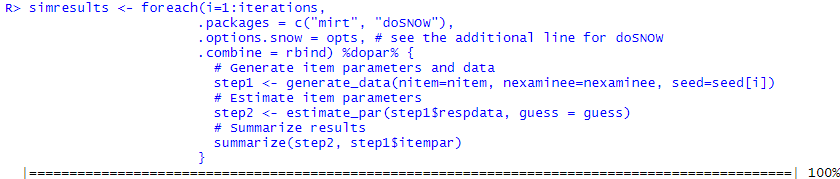
\includegraphics{figure/bench1.PNG}
\caption{Status of progress bar once the simulation is complete}
\end{figure}

\hypertarget{summarise}{%
\chapter{Summarizing Simulation Results}\label{summarise}}

\includegraphics{figure/fatos-bytyqi-Agx5_TLsIf4-unsplash.jpg}

\hypertarget{tables-and-figures}{%
\section{Tables and Figures}\label{tables-and-figures}}

\textbf{For plotting simulation results:}

\begin{itemize}
\tightlist
\item
  \texttt{ggplot2} \citep{R-ggplot2}
\item
  \texttt{lattice} \citep{R-lattice}
\item
  \texttt{plotly} \citep{R-plotly}
\end{itemize}

\textbf{For making tables with simulation results:}

\begin{itemize}
\tightlist
\item
  Check out \textbf{R Markdown}

  \begin{itemize}
  \tightlist
  \item
    RStudio guidelines for \texttt{R} Markdown: \url{https://rmarkdown.rstudio.com/}
  \item
    \texttt{R} Markdown: The Definitive Guide: \url{https://bookdown.org/yihui/rmarkdown/}
  \item
    Reproducible APA manuscripts with \texttt{R} Markdown: \url{https://crsh.github.io/papaja_man/reporting.html}
  \item
    HTML tables with \texttt{knitr::kable} and \texttt{kableExtra}: \url{http://haozhu233.github.io/kableExtra/}
  \item
    A nice blog post about stylish tables in \texttt{R}: \url{https://www.littlemissdata.com/blog/prettytables}
  \end{itemize}
\end{itemize}

\hypertarget{exporting-the-results}{%
\section{Exporting the Results}\label{exporting-the-results}}

I recommend exporting all the simulation results if:

\begin{itemize}
\tightlist
\item
  writing all the results into a file would not take a lot of space in the computer
\item
  existing computations are heavy and thus it is hard to summarize the results right away
\item
  it is likely that the simulation may be interrupted for some reason
\end{itemize}

Regardless what we decide to save (either all output or the summarized output), a nice way to save the results is to place a \texttt{write} function inside the loop. Using the nested \texttt{foreach} loops as an example, we will first create an empty .csv file called ``results.csv'':

\begin{Shaded}
\begin{Highlighting}[]
\KeywordTok{write.table}\NormalTok{(}\KeywordTok{matrix}\NormalTok{(}\KeywordTok{c}\NormalTok{(}\StringTok{"nitem"}\NormalTok{, }\StringTok{"nexaminee"}\NormalTok{, }\StringTok{"guess"}\NormalTok{, }\StringTok{"parameter"}\NormalTok{, }\StringTok{"bias"}\NormalTok{, }\StringTok{"rmse"}\NormalTok{, }\StringTok{"correlation"}\NormalTok{), }
                   \DataTypeTok{nrow =} \DecValTok{1}\NormalTok{, }
                   \DataTypeTok{ncol =} \DecValTok{7}\NormalTok{), }
            \DataTypeTok{file =} \StringTok{"results.csv"}\NormalTok{, }
            \DataTypeTok{sep =} \StringTok{","}\NormalTok{,}
            \DataTypeTok{col.names =} \OtherTok{FALSE}\NormalTok{, }
            \DataTypeTok{row.names =} \OtherTok{FALSE}\NormalTok{)}
\end{Highlighting}
\end{Shaded}

Then, we modify our code in a way that we will \textbf{not} save the results and instead write them into the results.csv file.

\begin{Shaded}
\begin{Highlighting}[]
\CommentTok{# Set all the conditions}
\NormalTok{iterations =}\StringTok{ }\DecValTok{100}
\NormalTok{seed =}\StringTok{ }\KeywordTok{sample.int}\NormalTok{(}\DecValTok{10000}\NormalTok{, }\DecValTok{100}\NormalTok{)}
\NormalTok{nitem =}\StringTok{ }\KeywordTok{c}\NormalTok{(}\DecValTok{10}\NormalTok{, }\DecValTok{15}\NormalTok{, }\DecValTok{20}\NormalTok{, }\DecValTok{25}\NormalTok{)}
\NormalTok{nexaminee =}\StringTok{ }\KeywordTok{c}\NormalTok{(}\DecValTok{250}\NormalTok{, }\DecValTok{500}\NormalTok{, }\DecValTok{750}\NormalTok{, }\DecValTok{1000}\NormalTok{)}
\NormalTok{guess =}\StringTok{ }\KeywordTok{c}\NormalTok{(}\OperatorTok{-}\DecValTok{1}\NormalTok{, }\FloatTok{0.16}\NormalTok{)}

\CommentTok{# Register four clusters}
\NormalTok{cl <-}\StringTok{ }\KeywordTok{makeCluster}\NormalTok{(}\DecValTok{4}\NormalTok{) }
\KeywordTok{registerDoParallel}\NormalTok{(cl)}

\CommentTok{# Run nested foreach loops}
\KeywordTok{foreach}\NormalTok{(}\DataTypeTok{i=}\DecValTok{1}\OperatorTok{:}\NormalTok{iterations, }
        \DataTypeTok{.packages =} \KeywordTok{c}\NormalTok{(}\StringTok{"mirt"}\NormalTok{, }\StringTok{"doParallel"}\NormalTok{, }\StringTok{"dplyr"}\NormalTok{),}
        \DataTypeTok{.combine =}\NormalTok{ rbind) }\OperatorTok
\StringTok{  }
\StringTok{  }\KeywordTok{foreach}\NormalTok{(}\DataTypeTok{j=}\NormalTok{nitem, }
          \DataTypeTok{.packages =} \KeywordTok{c}\NormalTok{(}\StringTok{"mirt"}\NormalTok{, }\StringTok{"doParallel"}\NormalTok{, }\StringTok{"dplyr"}\NormalTok{),}
          \DataTypeTok{.combine =}\NormalTok{ rbind)  }\OperatorTok
\StringTok{  }
\StringTok{ }\KeywordTok{foreach}\NormalTok{(}\DataTypeTok{k=}\NormalTok{nexaminee, }
          \DataTypeTok{.packages =} \KeywordTok{c}\NormalTok{(}\StringTok{"mirt"}\NormalTok{, }\StringTok{"doParallel"}\NormalTok{, }\StringTok{"dplyr"}\NormalTok{),}
          \DataTypeTok{.combine =}\NormalTok{ rbind)  }\OperatorTok
\StringTok{  }
\StringTok{  }\KeywordTok{foreach}\NormalTok{(}\DataTypeTok{m=}\NormalTok{guess, }
          \DataTypeTok{.packages =} \KeywordTok{c}\NormalTok{(}\StringTok{"mirt"}\NormalTok{, }\StringTok{"doParallel"}\NormalTok{, }\StringTok{"dplyr"}\NormalTok{),}
          \DataTypeTok{.combine =}\NormalTok{ rbind)  }\OperatorTok\StringTok{ }\NormalTok{\{}
            \CommentTok{# Generate item parameters and data}
\NormalTok{            step1 <-}\StringTok{ }\KeywordTok{generate_data}\NormalTok{(}\DataTypeTok{nitem=}\NormalTok{j, }\DataTypeTok{nexaminee=}\NormalTok{k, }\DataTypeTok{seed=}\NormalTok{seed[i])}
            \CommentTok{# Estimate item parameters}
\NormalTok{            step2 <-}\StringTok{ }\KeywordTok{estimate_par}\NormalTok{(step1}\OperatorTok{$}\NormalTok{respdata, }\DataTypeTok{guess =}\NormalTok{ m)}
            \CommentTok{# Summarize results}
\NormalTok{            step3 <-}\StringTok{ }\KeywordTok{summarize}\NormalTok{(step2, step1}\OperatorTok{$}\NormalTok{itempar)}
            \CommentTok{# Finalize results}
\NormalTok{            final <-}\StringTok{ }\NormalTok{step3 }\OperatorTok
\StringTok{              }\KeywordTok{group_by}\NormalTok{(parameter) }\OperatorTok
\StringTok{              }\KeywordTok{summarise}\NormalTok{(}\DataTypeTok{bias =} \KeywordTok{round}\NormalTok{(}\KeywordTok{mean}\NormalTok{(bias),}\DecValTok{3}\NormalTok{),}
                        \DataTypeTok{rmse =} \KeywordTok{round}\NormalTok{(}\KeywordTok{mean}\NormalTok{(rmse),}\DecValTok{3}\NormalTok{),}
                        \DataTypeTok{correlation =} \KeywordTok{round}\NormalTok{(}\KeywordTok{mean}\NormalTok{(correlation),}\DecValTok{3}\NormalTok{)) }\OperatorTok
\StringTok{              }\KeywordTok{mutate}\NormalTok{(}\DataTypeTok{nitem =}\NormalTok{ j,}
                     \DataTypeTok{nexaminee =}\NormalTok{ k,}
                     \DataTypeTok{guess =}\NormalTok{ m) }\OperatorTok
\StringTok{              }\KeywordTok{select}\NormalTok{(nitem, nexaminee, guess, parameter, bias, rmse, correlation) }\OperatorTok
\StringTok{              }\KeywordTok{as.data.frame}\NormalTok{()}
            \CommentTok{# Write the results}
            \KeywordTok{write.table}\NormalTok{(final, }\StringTok{"results.csv"}\NormalTok{, }
                        \DataTypeTok{sep =} \StringTok{","}\NormalTok{, }
                        \DataTypeTok{col.names =} \OtherTok{FALSE}\NormalTok{, }
                        \DataTypeTok{row.names =} \OtherTok{FALSE}\NormalTok{, }
                        \DataTypeTok{append =} \OtherTok{TRUE}\NormalTok{) }\CommentTok{# This will keep the file open for appending the results}
\NormalTok{            \}}

\CommentTok{# Stop the clusters}
\KeywordTok{stopCluster}\NormalTok{(cl)}
\end{Highlighting}
\end{Shaded}

  \bibliography{book.bib,packages.bib}

\end{document}
